\documentclass{report}

\usepackage[colorlinks=true, pdfstartview=FitV, linkcolor=xkcdBlue, citecolor=xkcdRed, urlcolor=xkcdGreen]{hyperref}
\usepackage{graphicx}
\usepackage{color}
\usepackage{amsmath}
\usepackage{hyperref}
\usepackage{enumerate}
\usepackage{xcolor}
\usepackage{xkcdcolors}
\usepackage{float}


% \addtolength{\topmargin}{-.7in}
% \addtolength{\textheight}{.6in}
\usepackage[a4paper, left=1.80cm, right=1.80cm, top=2cm, bottom=2cm, bindingoffset=0cm]{geometry} 



\begin{document}


\Large
\textbf{AE4868-II (2025/2026) - Assignment 1} \\
\normalsize \\

\emph{\textbf{Last update: \today}}\\

Name: Ismael Gallo López \\

Student number: 6541356 \\

Github link: \textit{\href{https://github.com/ismaelgallolopez/numerical-astrodynamics-GALLO_LOPEZ_Ismael}{https://github.com/ismaelgallolopez/numerical-astrodynamics-GALLO\_LOPEZ\_Ismael}} \\

Time spent per exercise:
\begin{enumerate}
    \item 7 h
    \item 6 h
    \item 6 h
    \item 13 h
\end{enumerate} 

People you worked with (if none, state this): 
\begin{itemize}
    \item Gemini 3
    \item Rodrigo Soares
    \item Andreu Craus Vidal
    \item Daniel Pérez Trías
    \item Gonzalo Guerrero Rodríguez
\end{itemize}

\clearpage

% KC: bold text here > bold text?

\section*{Question 1}

\subsection*{a}
% \textit{Insert figure}
\begin{figure}[H]
    \centering
    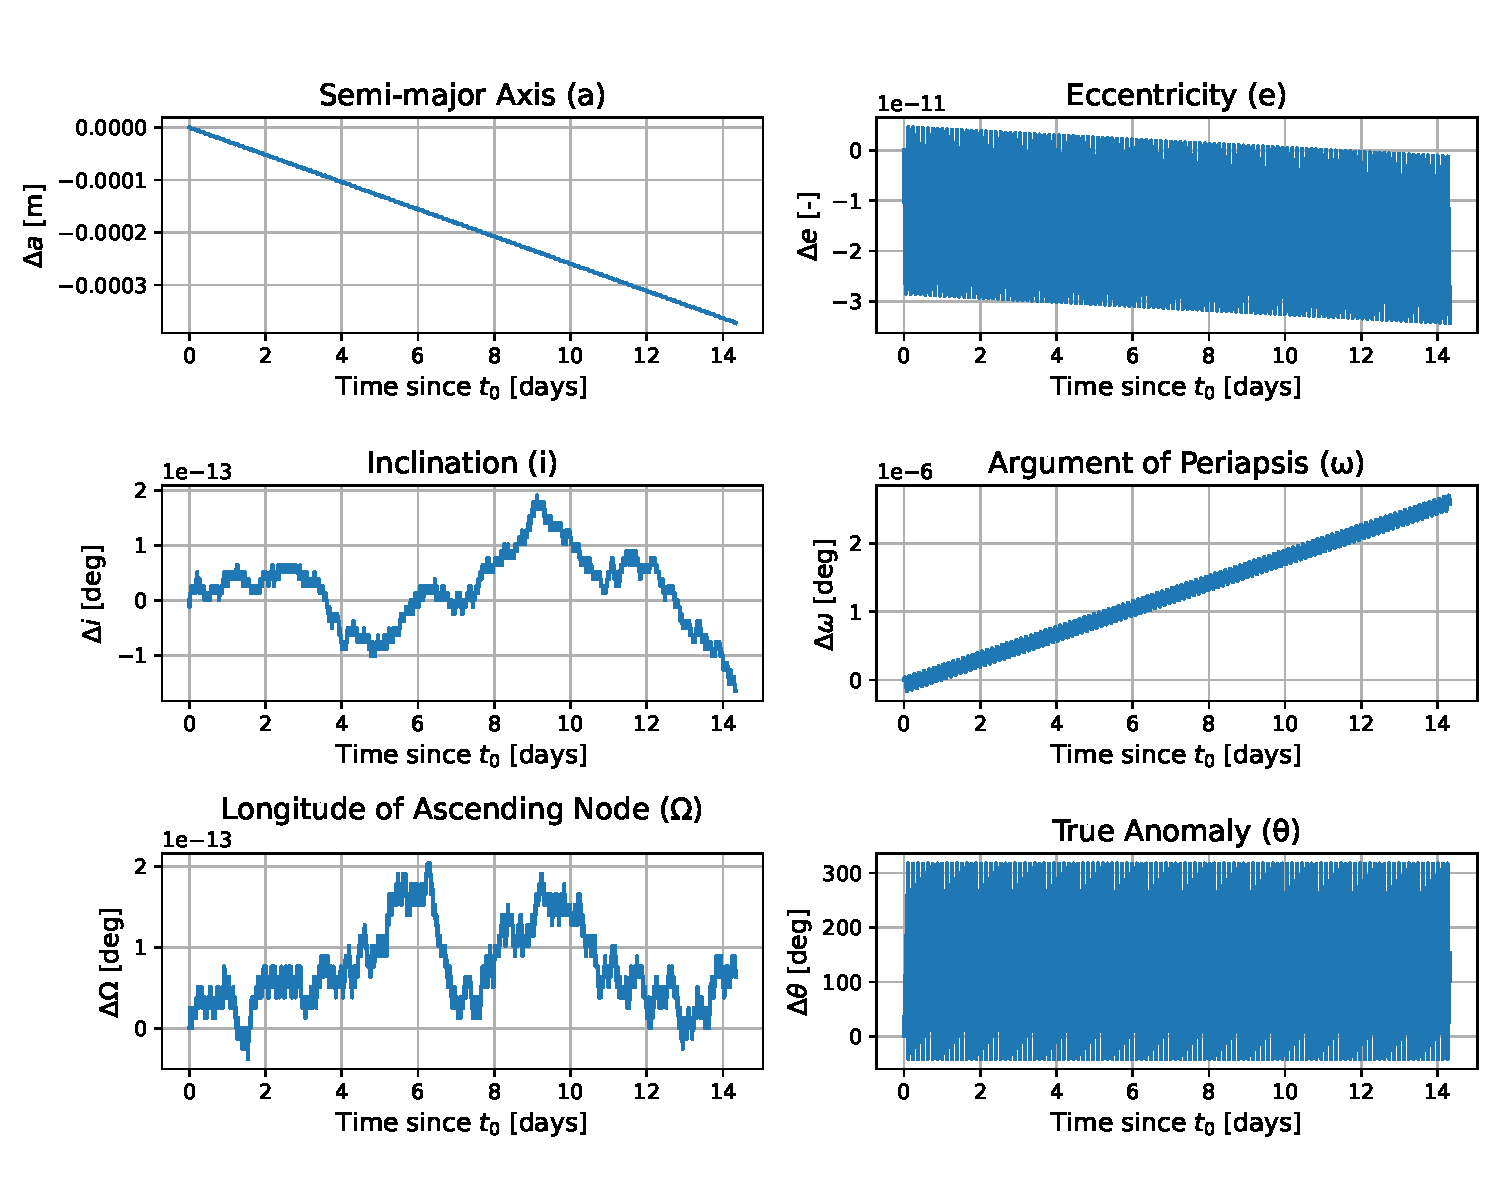
\includegraphics[width=0.85\textwidth]{../../figures/change_in_kepler_elements_q1.pdf}
    \caption{Change in Kepler elements of JUICE w.r.t $t_0$ (Frame: J2000)}
\end{figure}

\subsection*{b}
\begin{align}
    {\left(\mathbf{a}_{s}\right)_{G}}= -\frac{\mu_G}{\|\mathbf{r}_{Gs}\|^3} \mathbf{r}_{Gs}
\end{align}
where $\left(\mathbf{a}_{s}\right)_{G}$ is the Ganymede-centered acceleration of JUICE, $\mu_G$ is the gravitational parameter of Ganymede, and $\mathbf{r}_{Gs}$ is the position vector from Ganymede to JUICE.

\subsection*{c}
Positions from environment: initial position $\mathbf{r}_{Gs}(t=0)$ \\
Positions from numerical propagation: every other position $\mathbf{r}_{Gs}(t>0)$

\subsection*{d}
\begin{figure}[H]
    \centering
    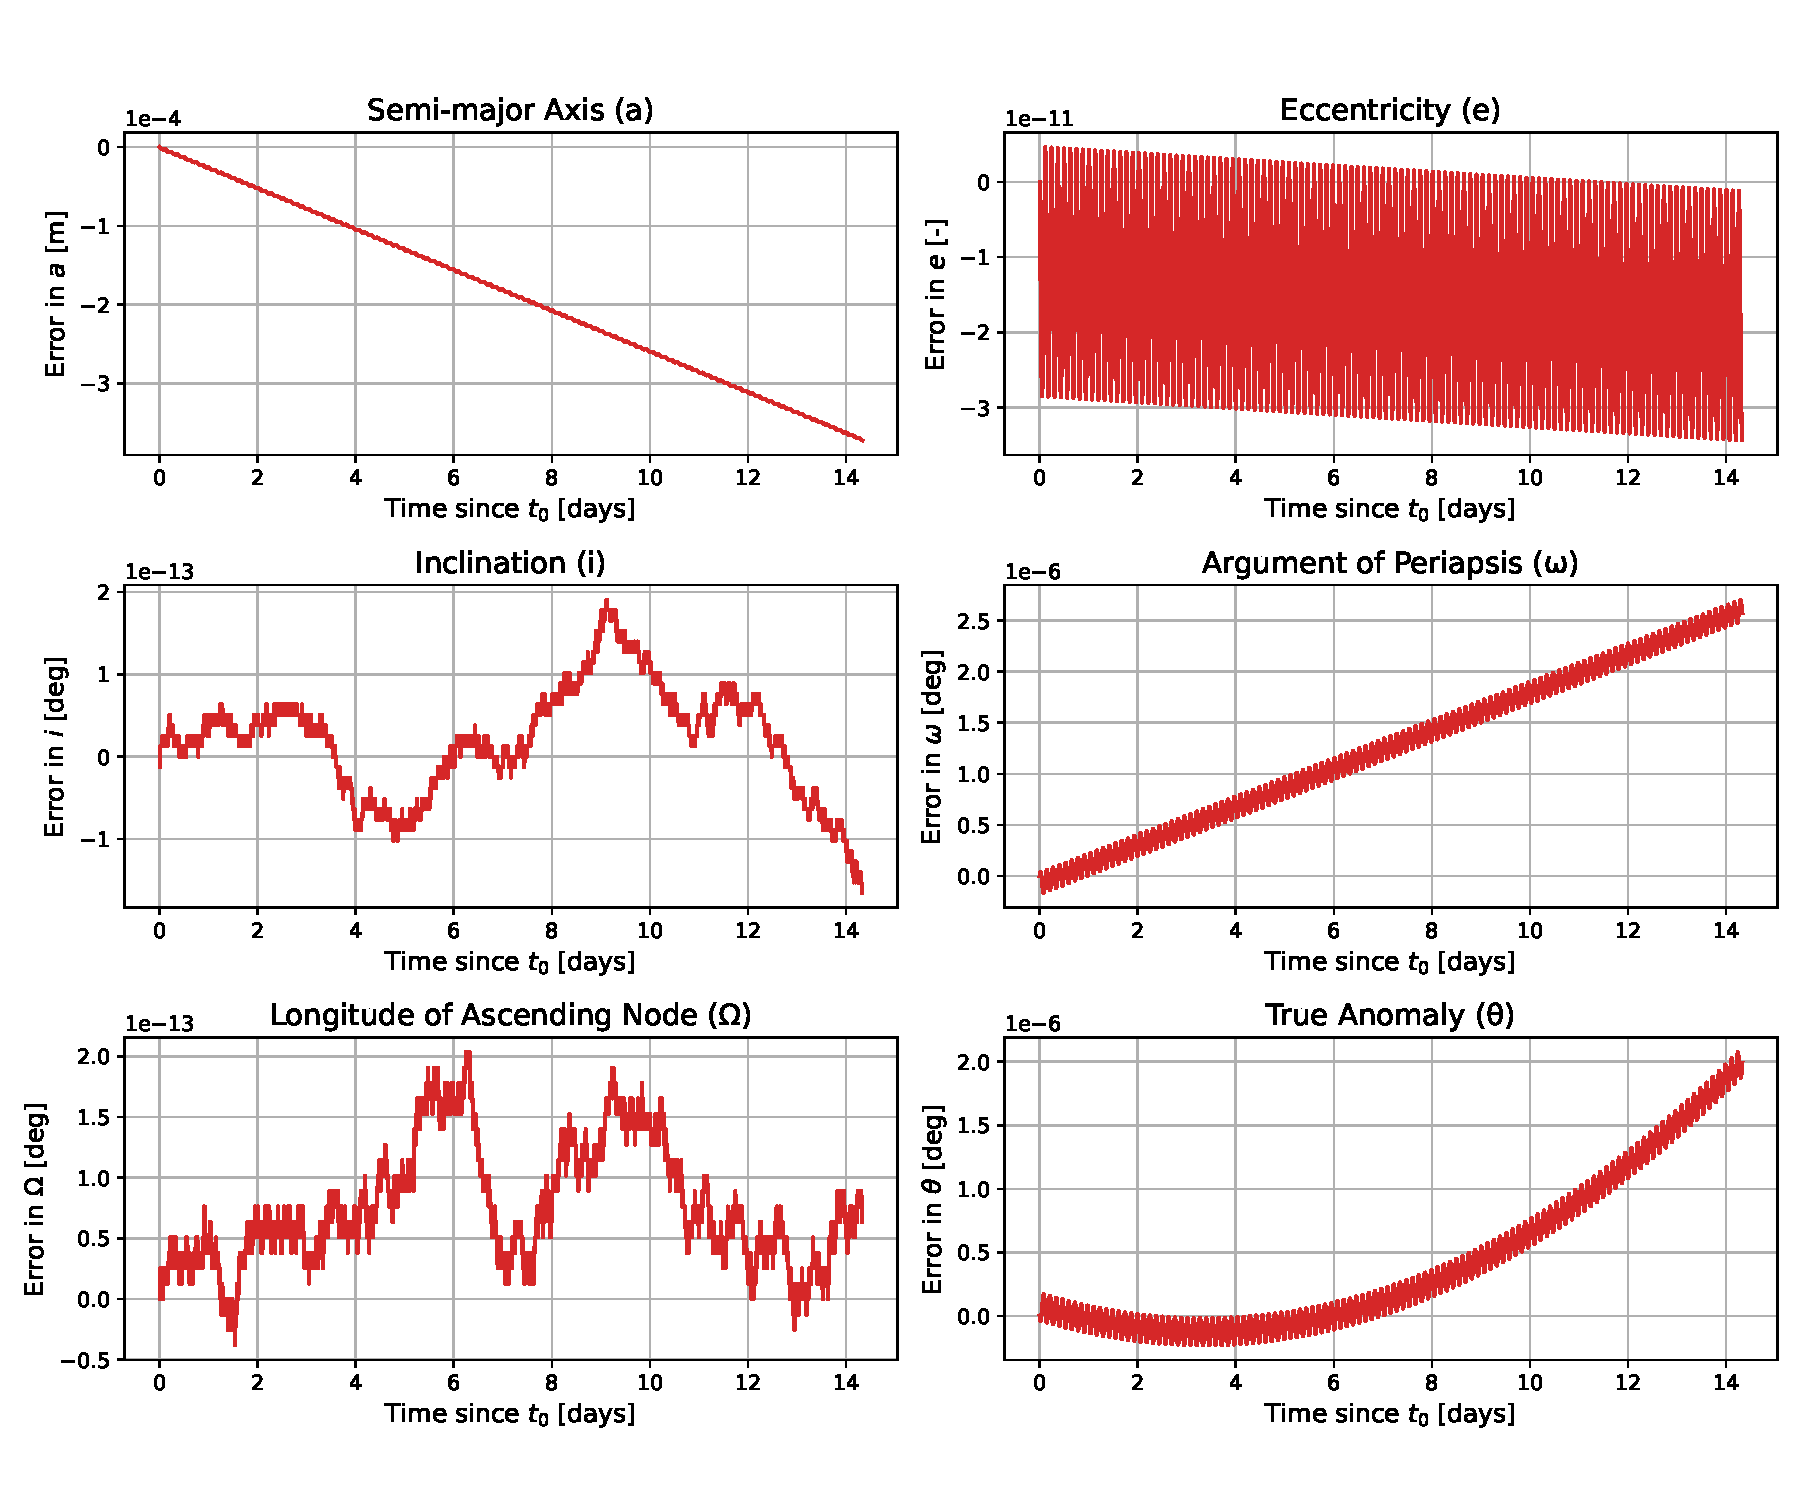
\includegraphics[width=0.85\textwidth]{../../figures/keplerian_integration_error_q1.pdf}
    \caption{Numerical Integration Error vs Analytical Solution (Keplerian)}
\end{figure}

\begin{figure}[H]
    \centering
    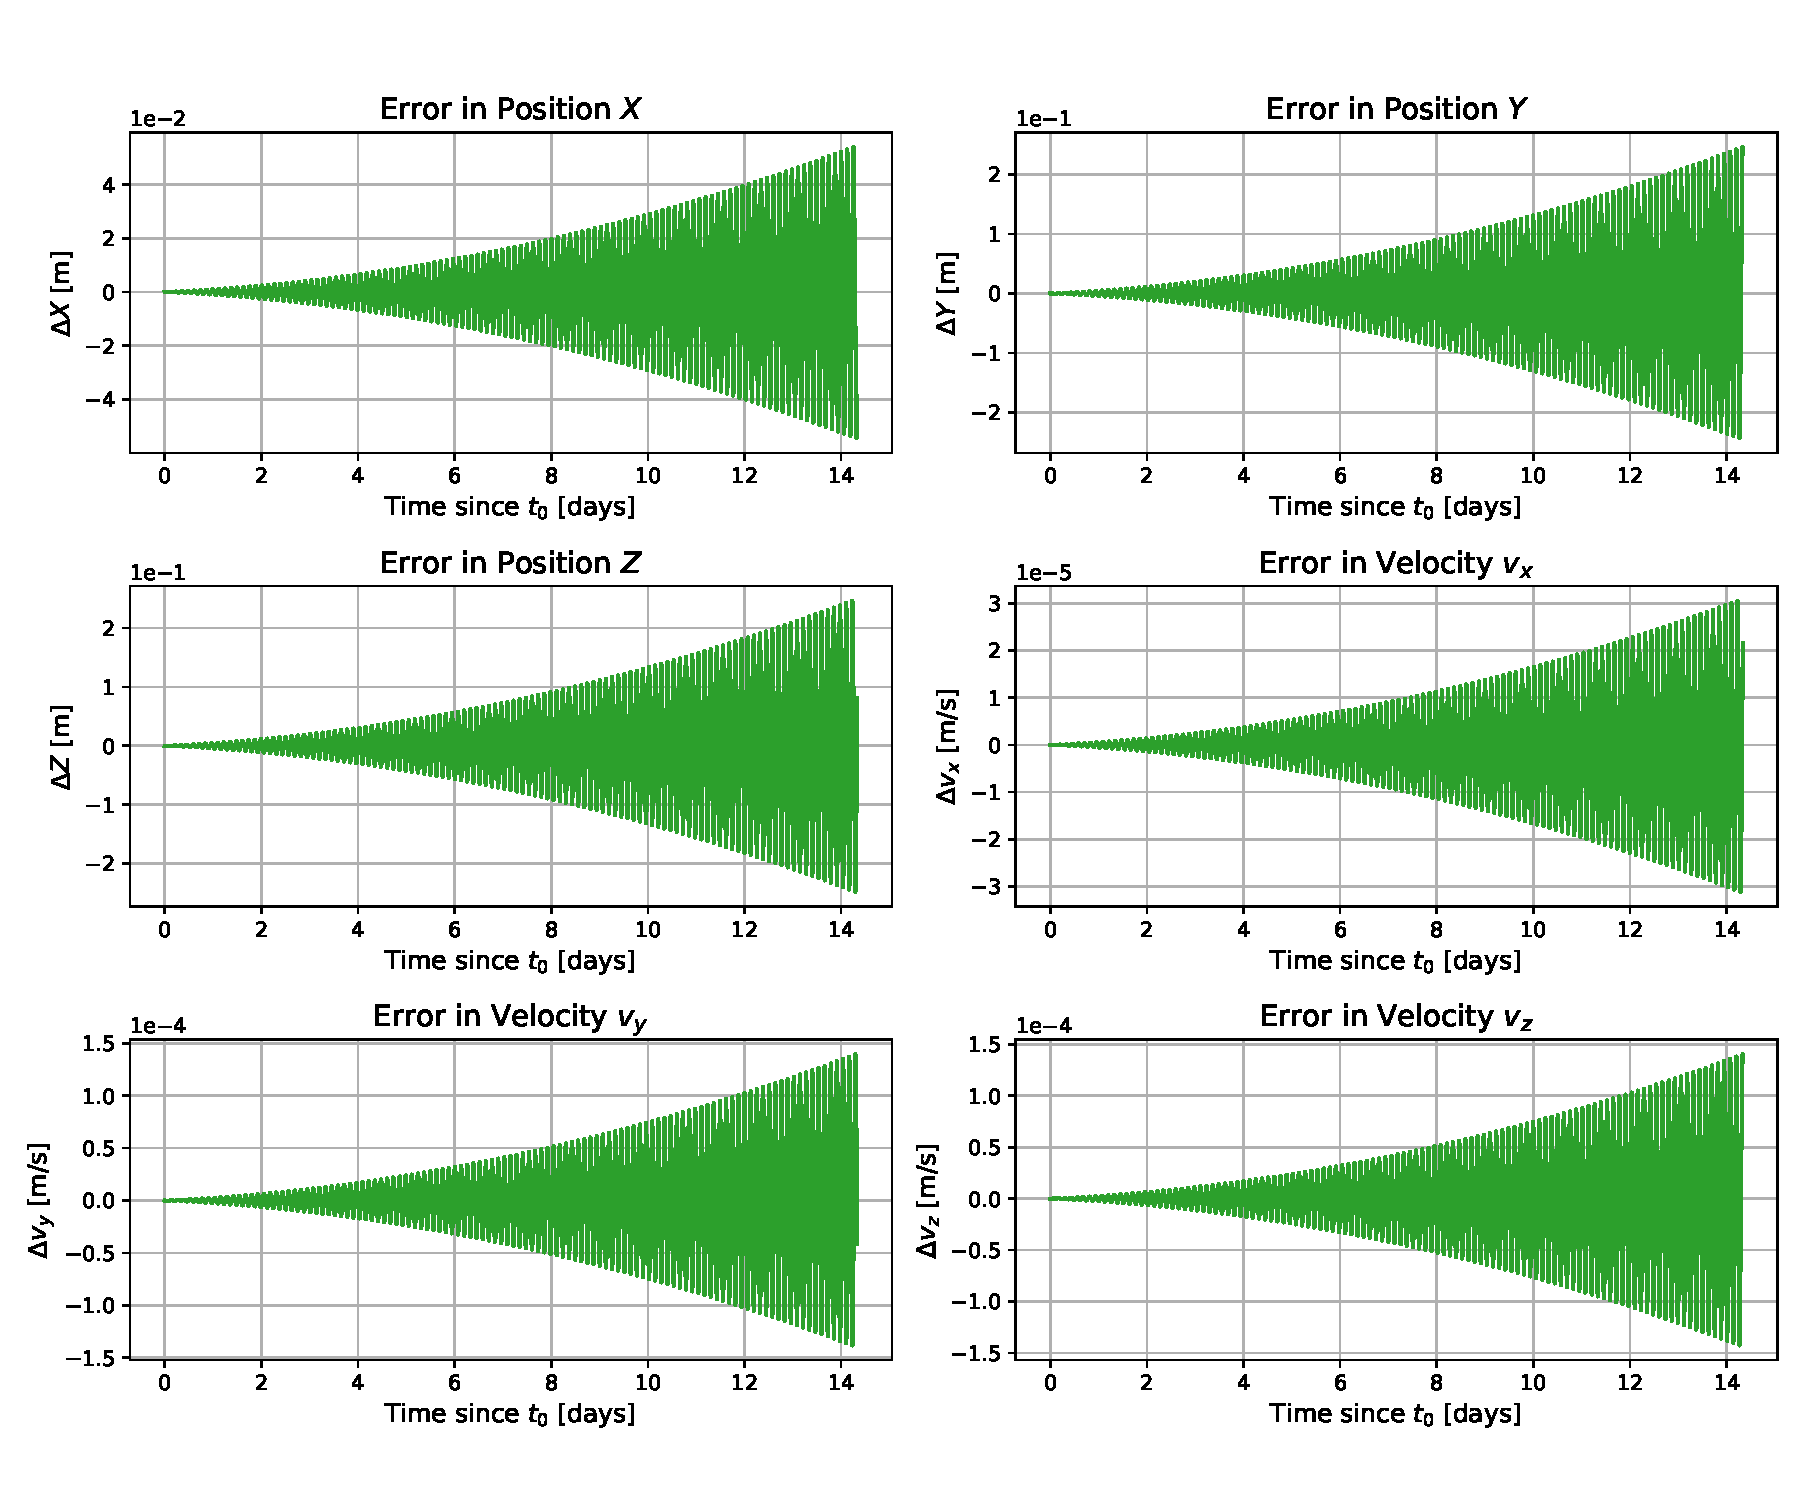
\includegraphics[width=0.85\textwidth]{../../figures/cartesian_integration_error_q1.pdf}
    \caption{Numerical Integration Error vs Analytical Solution (Cartesian)}
\end{figure}

\clearpage
\section*{Question 2}

\subsection*{a}
\begin{gather*}
    \left(\mathbf{a}_{G,s}\right)_{G} = \nabla U_G (\mathbf{r}_{Gs}) \\ 
    \left(\mathbf{a}_{J,s}\right)_{G} = \nabla U_J (\mathbf{r}_{Js}) - \nabla U_J (\mathbf{r}_{JG}) = \nabla U_J (\mathbf{r}_{JG} + \mathbf{r}_{Gs}) - \nabla U_J (\mathbf{r}_{JG}) \\
    \left(\mathbf{a}_{I,s}\right)_{G} = -\frac{\mu_I}{\|\mathbf{r}_{Is}\|^3} \mathbf{r}_{Is} - \left( - \mu_I \frac{\mathbf{r}_{IG}}{\|\mathbf{r}_{IG}\|^3} \right) 
                                      = -\mu_I \left( \frac{\mathbf{r}_{IG} + \mathbf{r}_{Gs}}{\|\mathbf{r}_{IG} + \mathbf{r}_{Gs}\|^3} - \frac{\mathbf{r}_{IG}}{\|\mathbf{r}_{IG}\|^3} \right) \\
\end{gather*}
where $\left(\mathbf{a}_{G,s}\right)_{G}$ is the Ganymede-centered acceleration of JUICE due to Ganymede, $U_G$ is the gravitational potential of Ganymede, $\mathbf{r}_{Gs}$ is the position vector from Ganymede to JUICE, $\left(\mathbf{a}_{J,s}\right)_{G}$ is the Ganymede-centered acceleration of JUICE due to Jupiter, $U_J$ is the gravitational potential of Jupiter, $\mathbf{r}_{Js}$ is the position vector from Jupiter to JUICE, $\mathbf{r}_{JG}$ is the position vector from Jupiter to Ganymede, $\left(\mathbf{a}_{I,s}\right)_{G}$ is the Ganymede-centered acceleration of JUICE due to Io, $\mu_I$ is the gravitational parameter of Io, $\mathbf{r}_{Is}$ is the position vector from Io to JUICE, and $\mathbf{r}_{IG}$ is the position vector from Io to Ganymede.

\subsection*{b}
Positions from environment: 
% initial position of JUICE
$\mathbf{r}_{Gs}(t=0)$; 
% position of every other celestial body at every instant:
$\mathbf{r}_{IG}$, $\mathbf{r}_{JG}$ \\
Positions from numerical propagation: 
% every other position of JUICE
 $\mathbf{r}_{Gs}(t>0)$

\subsection*{c.i}

\begin{figure}[H]
    \centering
    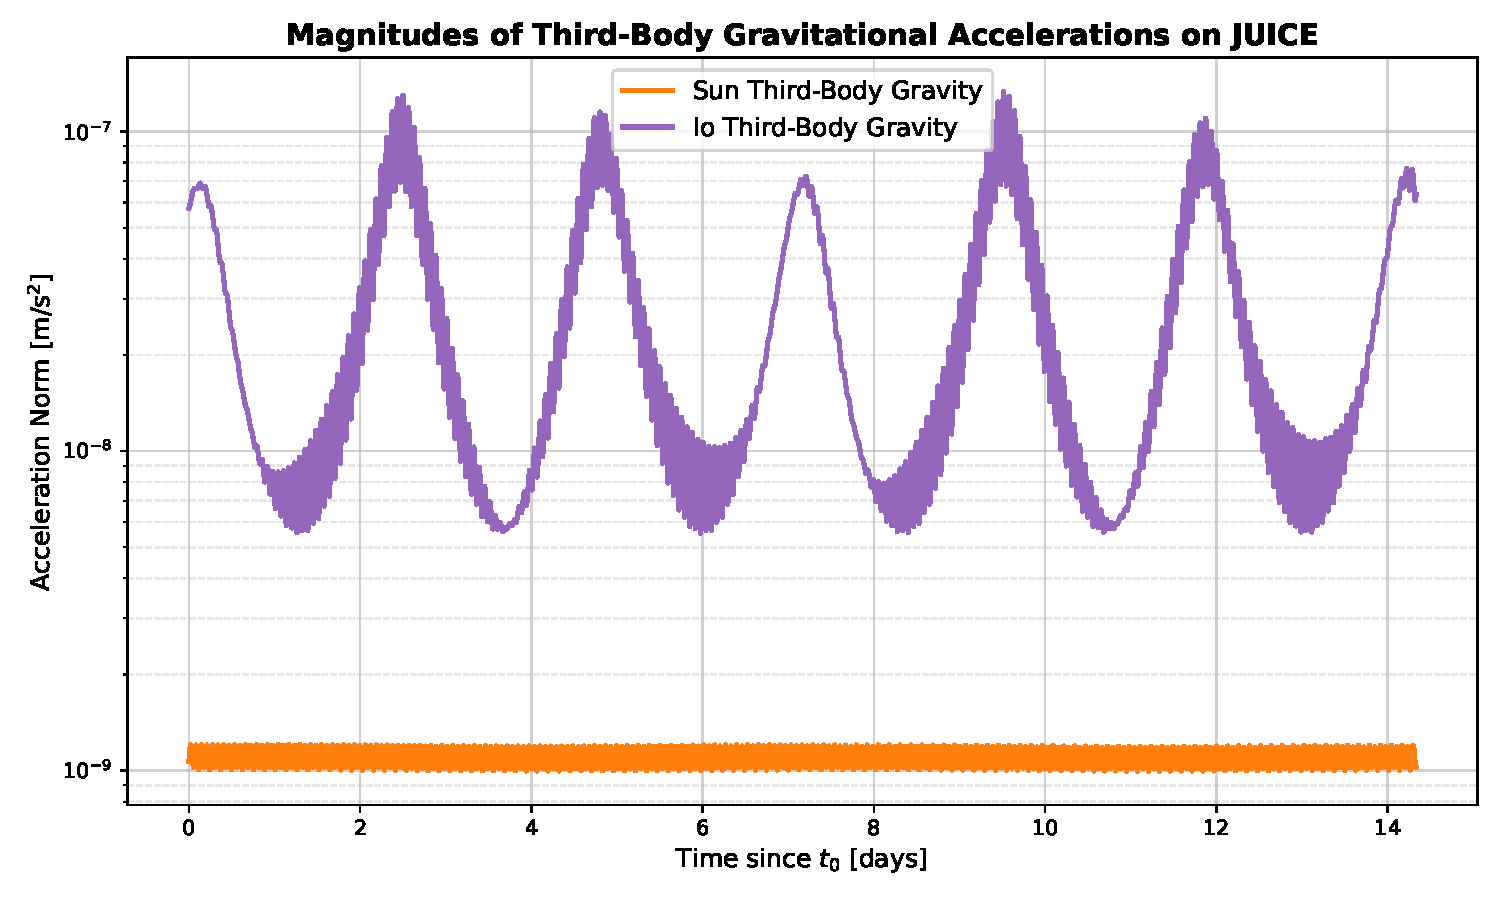
\includegraphics[width=0.85\textwidth]{../../figures/third_body_accelerations_q2.pdf}
    \caption{Ganymede-centered gravitational accelerations acting on JUICE due to Io (purple) and the Sun (orange).}
\end{figure}

\subsection*{c.ii}

\begin{equation}
    T_{\text{max,Io}}\approx 57.33~\text{hr} = 2.39~\text{days}
    \quad\mathrm{and}\quad 
    T_{\text{max,Sun}}\approx 1.53~\text{hr} = 0.06~\text{days}
\end{equation}
where $T_{\text{max,Io}}$ is the period of maximum amplitude for Io-induced acceleration and $T_{\text{max,Sun}}$ is the period of maximum amplitude for Sun-induced acceleration.

\begin{figure}[H]
    \centering
    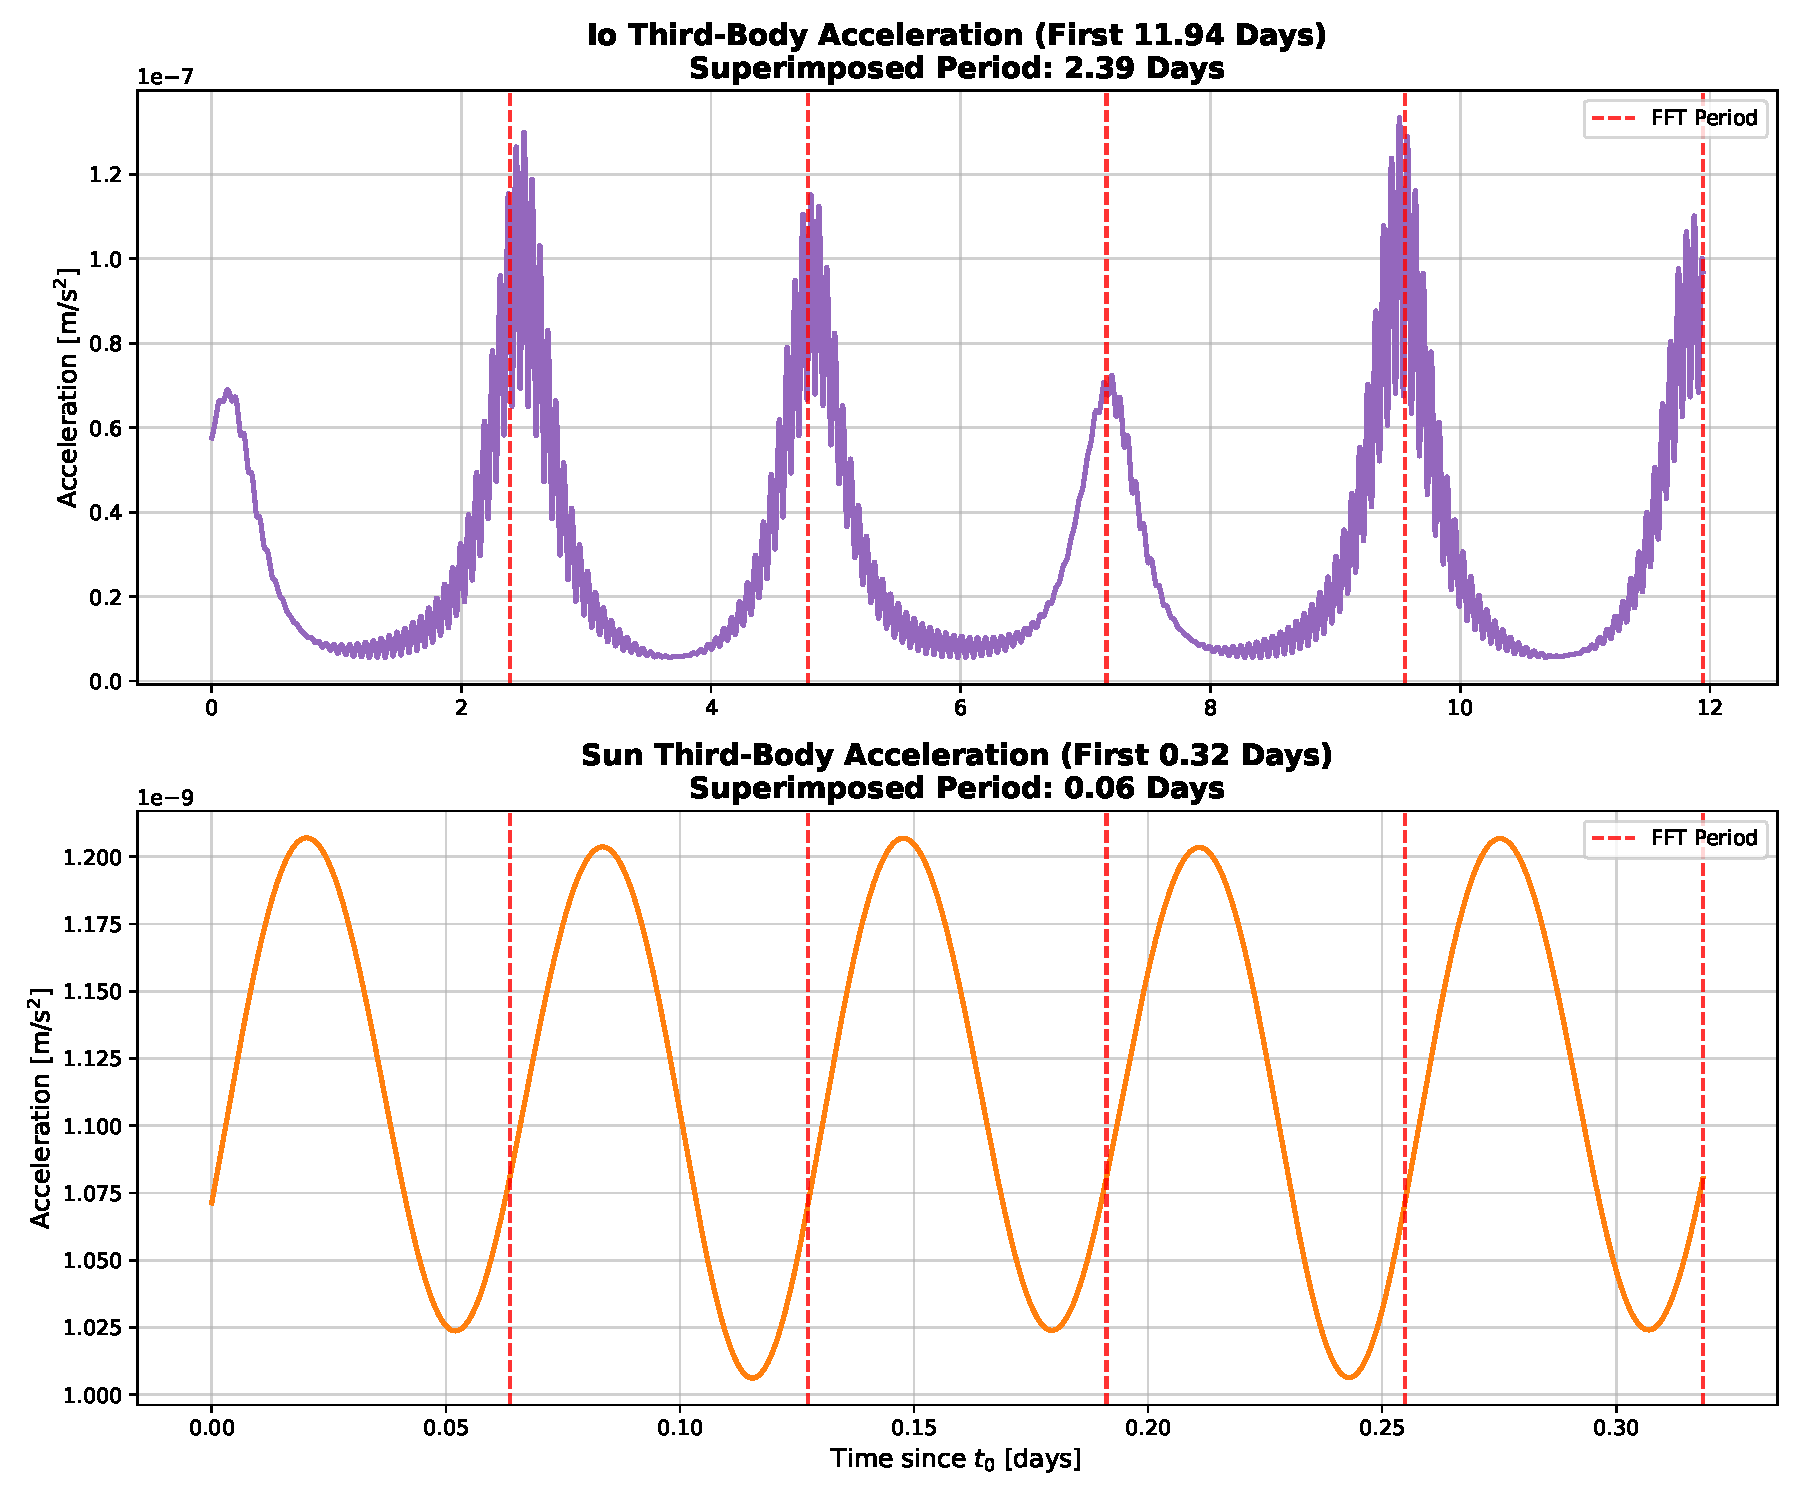
\includegraphics[width=0.85\textwidth]{../../figures/zoomed_accelerations_periods_q2.pdf}
    \caption{Ganymede-centered gravitational accelerations (zoomed for detail) acting on JUICE due to Io (purple) and the Sun (orange), with the period of the acceleration with the largest amplitude superposed.}
\end{figure}

% \footnote{No figures used, the answer is extracted from the FFT of the accelerations done with SciPy library.}
% \textit{Insert figure(s) to support your explanation, and \textbf{explain briefly why this figure leads to the answer you fill in above}}

\subsection*{c.iii}

\begin{equation}
    T_{\text{max,Io}}=\frac{1}{3} T_{G} = \frac{4}{3} T_{I} 
    \quad\mathrm{and}\quad 
    T_{\text{max,Sun}}= \frac{1}{2} T_{\text{JUICE}} 
\end{equation}
where $T_{G}$ is the orbital period of Ganymede, $T_{I}$ is the orbital period of Io, and $T_{\text{JUICE}}$ is the orbital period of JUICE around Ganymede.

\subsection*{c.iv}

% \textit{\textbf{Answer on physical reason for Io-induced period.} (be brief)}  \\
% \textit{\textbf{Answer on physical reason for Sun-induced period.}}  

The gravitational perturbation from Io is primarily driven by the Io-Ganymede synodic period. In the Ganymede-centered frame, this acceleration reaches its maximum during conjunction and its minimum when Io is in quadrature ($90^\circ$ offset).
\footnote{\url{https://upload.wikimedia.org/wikipedia/commons/8/83/Galilean_moon_Laplace_resonance_animation.gif}} 

Conversely, the solar perturbation can be analyzed by treating the Sun-Ganymede vector as quasi-static, ($T_{Ganymede} \gg T_{JUICE}$). The resulting acceleration on JUICE depends on its alignment relative to the Sun-Ganymede axis.  This effect peaks when the spacecraft is collinear with the Sun and minimizes when the position vector is orthogonal to the Sun-Ganymede line. Consequently, this geometry results in two maxima per revolution.

\subsection*{c.v}

\begin{equation*}
    \left(\mathbf{a}_{S,s}\right)_{G} = -\mu_{S} \left( \frac{\mathbf{r}_{Ss}}{||\mathbf{r}_{Ss}||^3} - \frac{\mathbf{r}_{SG}}{||\mathbf{r}_{SG}||^3} \right)
\end{equation*}
where $\left(\mathbf{a}_{S,s}\right)_{G}$ is the Ganymede-centered acceleration of JUICE due to the Sun, $\mu_{S}$ is the gravitational parameter of the Sun, $\mathbf{r}_{Ss}$ is the position vector from the Sun to JUICE, and $\mathbf{r}_{SG}$ is the position vector from the Sun to Ganymede.

Assupmtions:
\begin{enumerate}
    \item $||\mathbf{r}_{SG}|| \gg ||\mathbf{r}_{Gs}||$ 
    
    {Sun-Ganymede distance is much larger than the spacecraft's orbital radius.}\\
    \item $||\mathbf{r}_{SG}|| \approx \text{constant}$ 
    
    {Ganymede’s heliocentric distance is constant over JUICE’s orbital period.}\\
    \item $(1+x)^{-3/2} \approx 1 - \frac{3}{2}x$ (first order Taylor expansion)
    
    {First-order Taylor expansion applies to the small ratio of orbital distances.}\\
\end{enumerate}

Derivation steps:
\begin{enumerate}
    % \textbf{Derivation step   1 (Assumption 1):}\\
    \item $\mathbf{r}_{Ss} = \mathbf{r}_{SG} + \mathbf{r}_{Gs}$
    
    {Express the Sun-spacecraft vector as the sum of relative position vectors.}\\
    % \textbf{Derivation step 2 (Assumption 1):}\\
    \item $\left(\mathbf{a}_{S,s}\right)_{G} = -\mu_{S} \left( \frac{\mathbf{r}_{SG} + \mathbf{r}_{Gs}}{||\mathbf{r}_{SG} + \mathbf{r}_{Gs}||^3} - \frac{\mathbf{r}_{SG}}{||\mathbf{r}_{SG}||^3} \right)$
    
    {Substitute the vector sum into the relative acceleration formula.}\\
    % \textbf{Derivation step 3 (Assumption 1):}\\
    \item $||\mathbf{r}_{SG} + \mathbf{r}_{Gs}||^{-3} = \left( ||\mathbf{r}_{SG}||^2 + 2\mathbf{r}_{SG} \cdot \mathbf{r}_{Gs} + ||\mathbf{r}_{Gs}||^2 \right)^{-3/2}$ 
    
    {Expand the magnitude of the Sun-spacecraft vector using the law of cosines ($ \mathbf{r}_{SG} \cdot \mathbf{r}_{Gs} = ||\mathbf{r}_{SG}|| ||\mathbf{r}_{Gs}|| \cos\theta $).}\\
    % \textbf{Derivation step 4 (Assumption 1, 3):}\\
    \item $||\mathbf{r}_{SG} + \mathbf{r}_{Gs}||^{-3} \approx ||\mathbf{r}_{SG}||^{-3} \left( 1 - 3 \frac{||\mathbf{r}_{Gs}||}{||\mathbf{r}_{SG}||} \cos\theta \right)$ 
    
    {Factor $||\mathbf{r}_{SG}||$, apply binomial expansion and neglect higher-order terms.}\\
    % \textbf{Derivation step 5 (Assumption 1):}\\
    \item $\left(\mathbf{a}_{S,s}\right)_{G} \approx -\frac{\mu_{S}}{||\mathbf{r}_{SG}||^3} \left[ (\mathbf{r}_{SG} + \mathbf{r}_{Gs}) \left( 1 - 3 \frac{||\mathbf{r}_{Gs}||}{||\mathbf{r}_{SG}||} \cos\theta \right) - \mathbf{r}_{SG} \right]$ 
    
    {Substitute the linearized magnitude back into the acceleration equation.}\\
    % \textbf{Derivation step 6 (Assumption 1, 2):}\\
    \item $||\left(\mathbf{a}_{S,s}\right)_{G}|| \approx \frac{\mu_{S} ||\mathbf{r}_{Gs}||}{||\mathbf{r}_{SG}||^3} \sqrt{1 + 3\cos^2\theta}$ 
    
    {Simplify the magnitude as a function of the Sun-Ganymede relative angle.}\\
\end{enumerate}

The acceleration magnitude depends on $\cos^2\theta$, which reaches a maximum twice per orbit (at $\theta = 0^\circ$ and $180^\circ$). 
\clearpage

\section*{Question 3}
\subsection*{a}

\begin{align}
    \mathbf{a}_{\text{Aero}}= -\frac{1}{m} \left( \frac{1}{2} \rho v_{air}^2 C_D S_{ref} \right) \mathbf{\hat{v}_{air}} = -\frac{1}{m} \left( q_{air} C_D S_{ref} \right) \mathbf{\hat{v}_{air}} \\
    \mathbf{a}_{\text{SRP}}= \left( \frac{P}{4 \pi c} \right) \left( \frac{C_r S_{ref}}{m} \right) \frac{\mathbf{r}_{Ss}}{\|\mathbf{r}_{Ss}\|^3}
\end{align}
where $\mathbf{a}_{\text{Aero}}$ is the aerodynamic acceleration, $m$ is the spacecraft mass, $\rho$ is the atmospheric density, $v_{air}$ is the airspeed magnitude, $C_D$ is the drag coefficient, $S_{ref}$ is the reference area, $\mathbf{\hat{v}_{air}}$ is the unit vector in the airspeed direction, $q_{air}$ is the dynamic pressure, $\mathbf{a}_{\text{SRP}}$ is the solar radiation pressure acceleration, $P$ is the solar luminosity, $c$ is the speed of light, $C_r$ is the radiation pressure coefficient, and $\mathbf{r}_{Ss}$ is the position vector from the Sun to JUICE.

\begin{figure}[H]
    \centering
    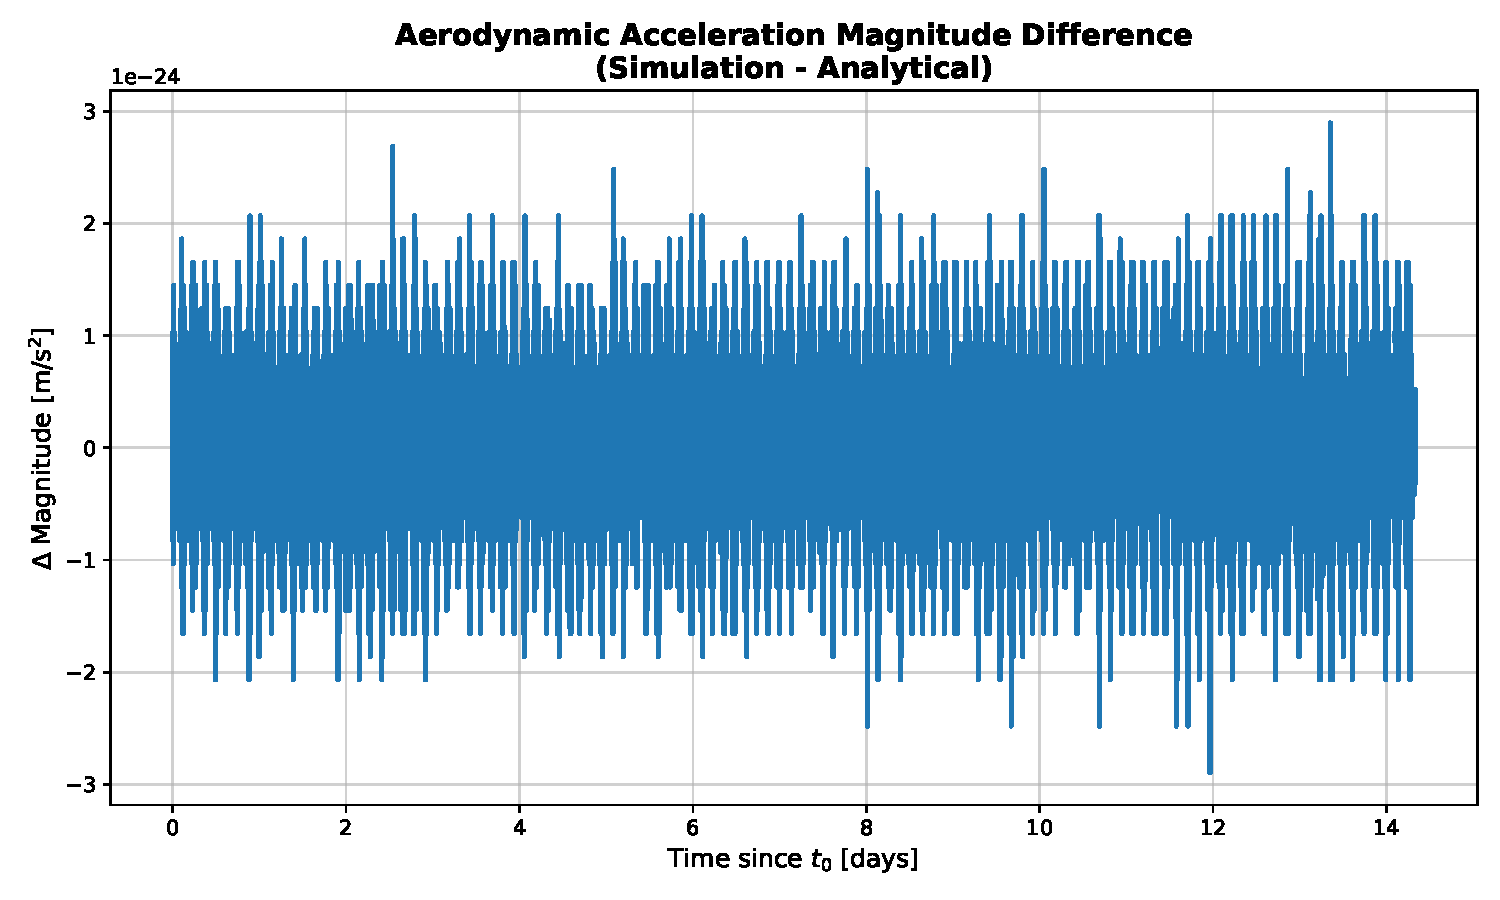
\includegraphics[width=0.85\textwidth]{../../figures/validation_aero_mag_diff_q3.pdf}
    \caption{Difference in Ganymede-centered aerodynamic acceleration magnitude acting on JUICE, between manually calculated and extracted from propagation.}
    \label{fig:aero_mag_diff_q3}
\end{figure}

\begin{figure}[H]
    \centering
    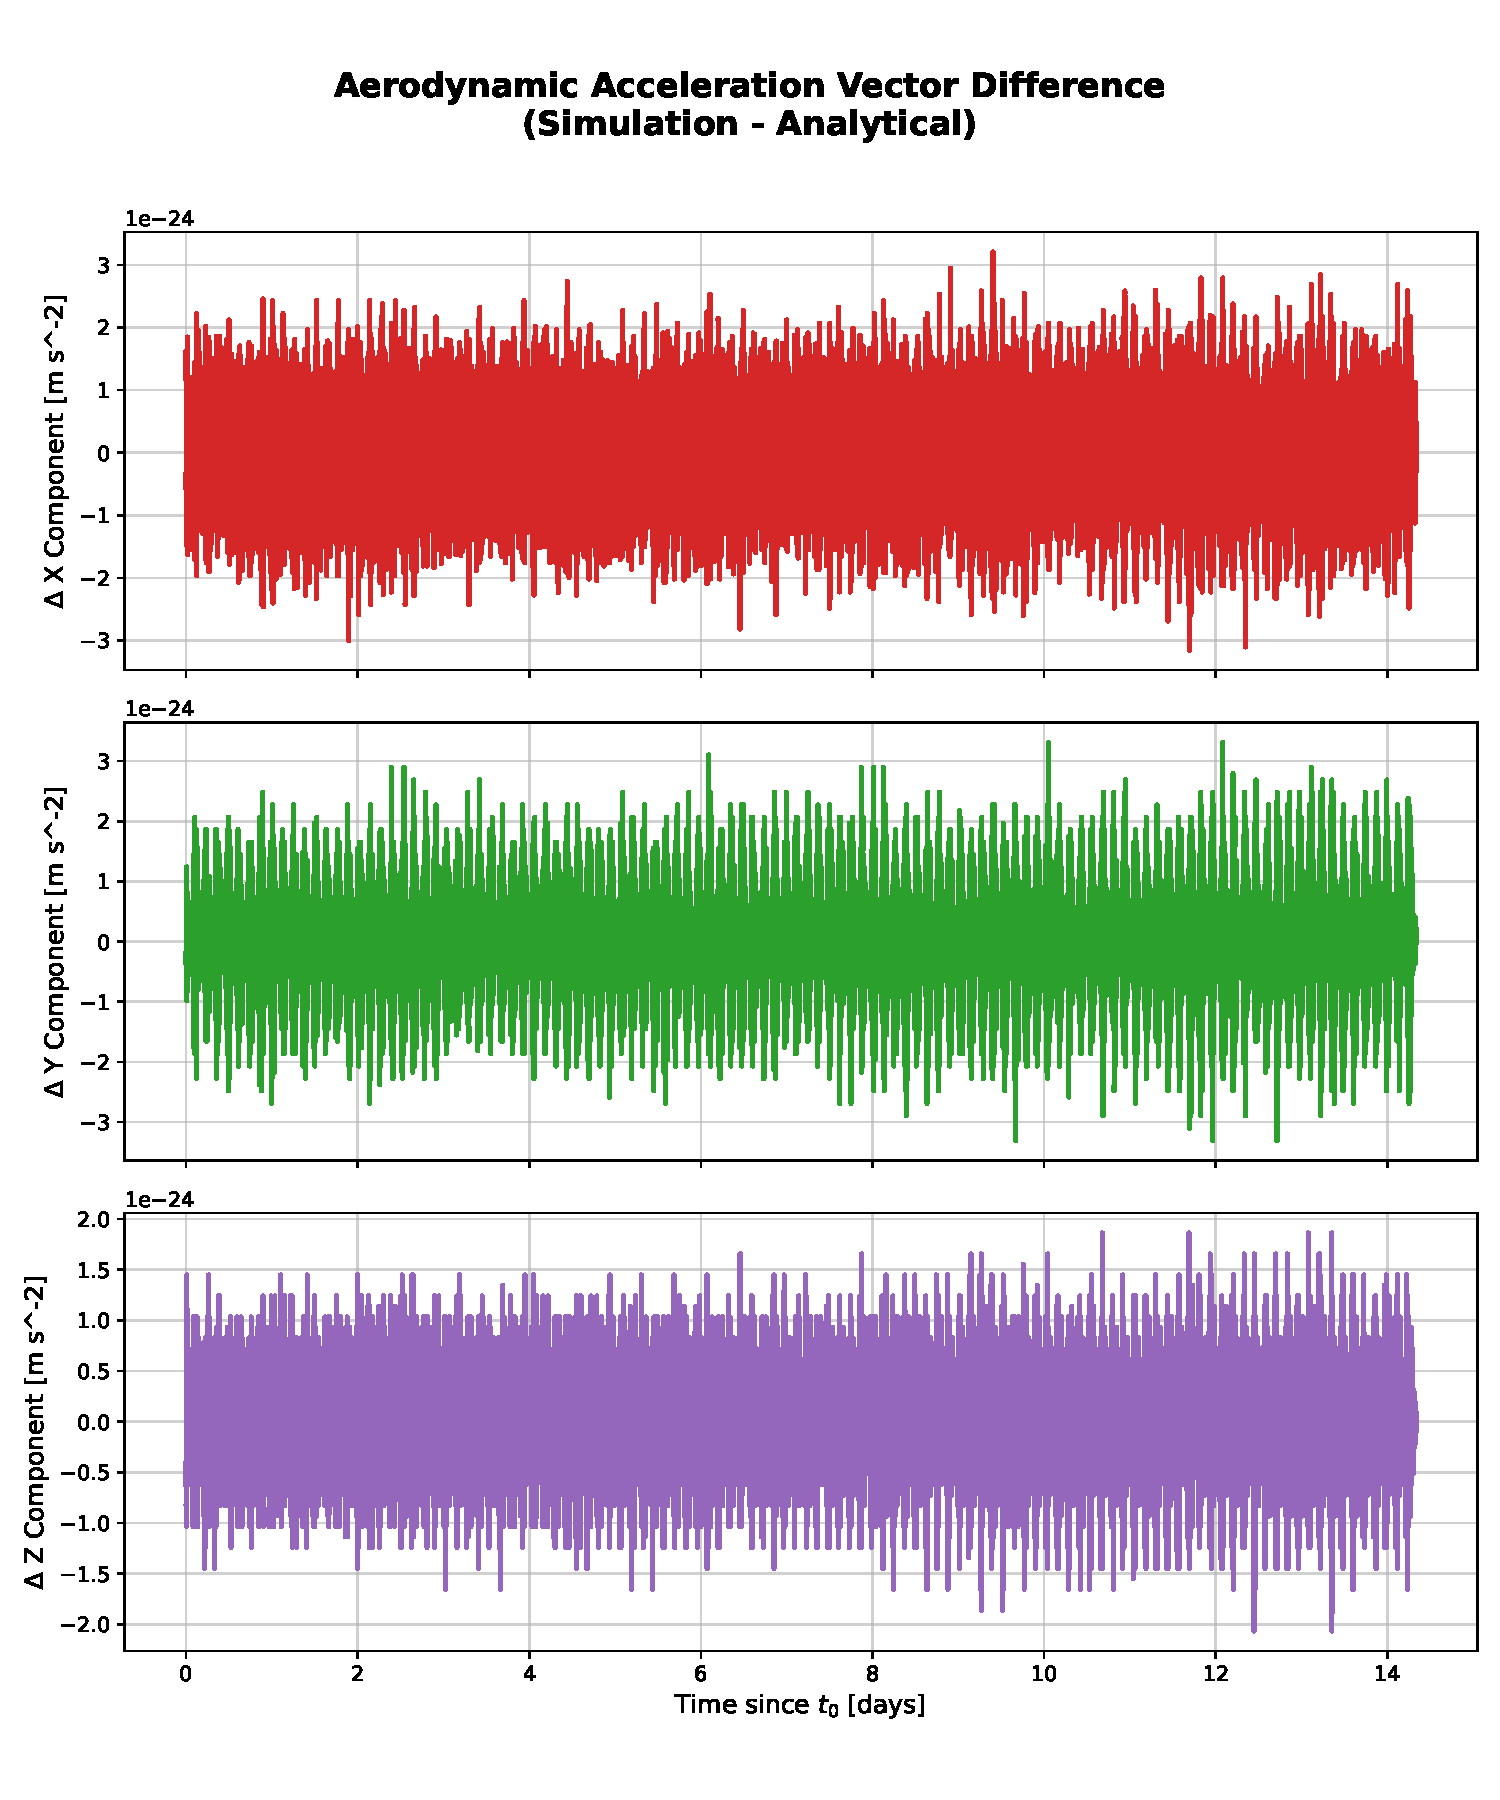
\includegraphics[width=0.85\textwidth]{../../figures/validation_aero_vector_diff_q3.pdf}
    \caption{Difference in Ganymede-centered aerodynamic acceleration vector acting on JUICE, between manually calculated and extracted from propagation.}
    \label{fig:aero_vector_diff_q3}
\end{figure}

\begin{figure}[H]
    \centering
    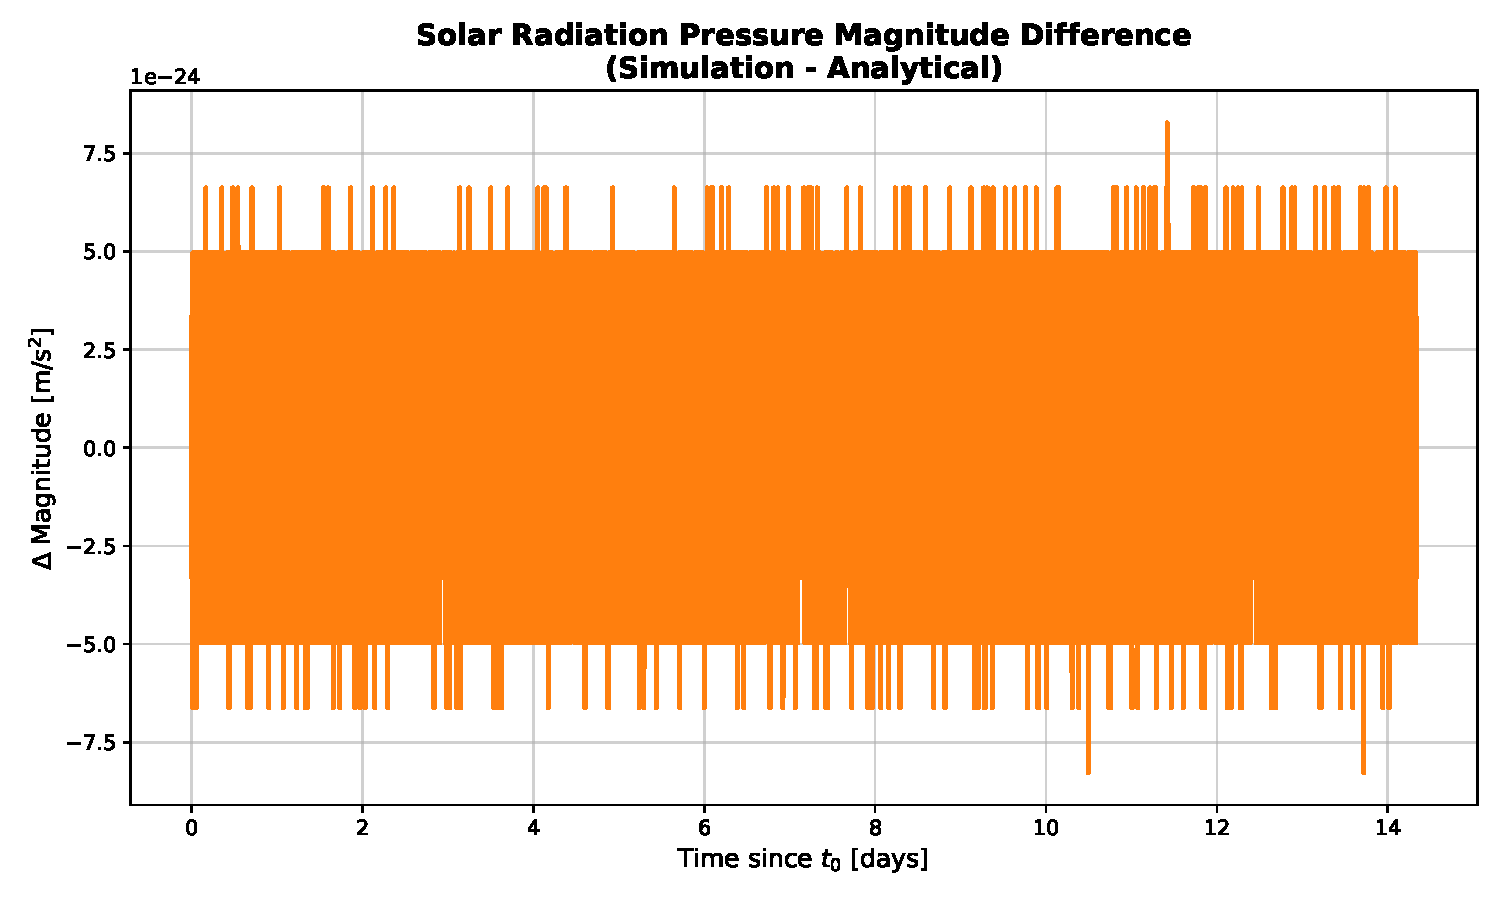
\includegraphics[width=0.85\textwidth]{../../figures/validation_srp_mag_diff_q3.pdf}
    \caption{Difference in Ganymede-centered Solar Radiation Pressure acceleration magnitude acting on JUICE, between manually calculated and extracted from propagation}
    \label{fig:validation_srp_mag_diff_q3}
\end{figure}

\begin{figure}[H]
    \centering
    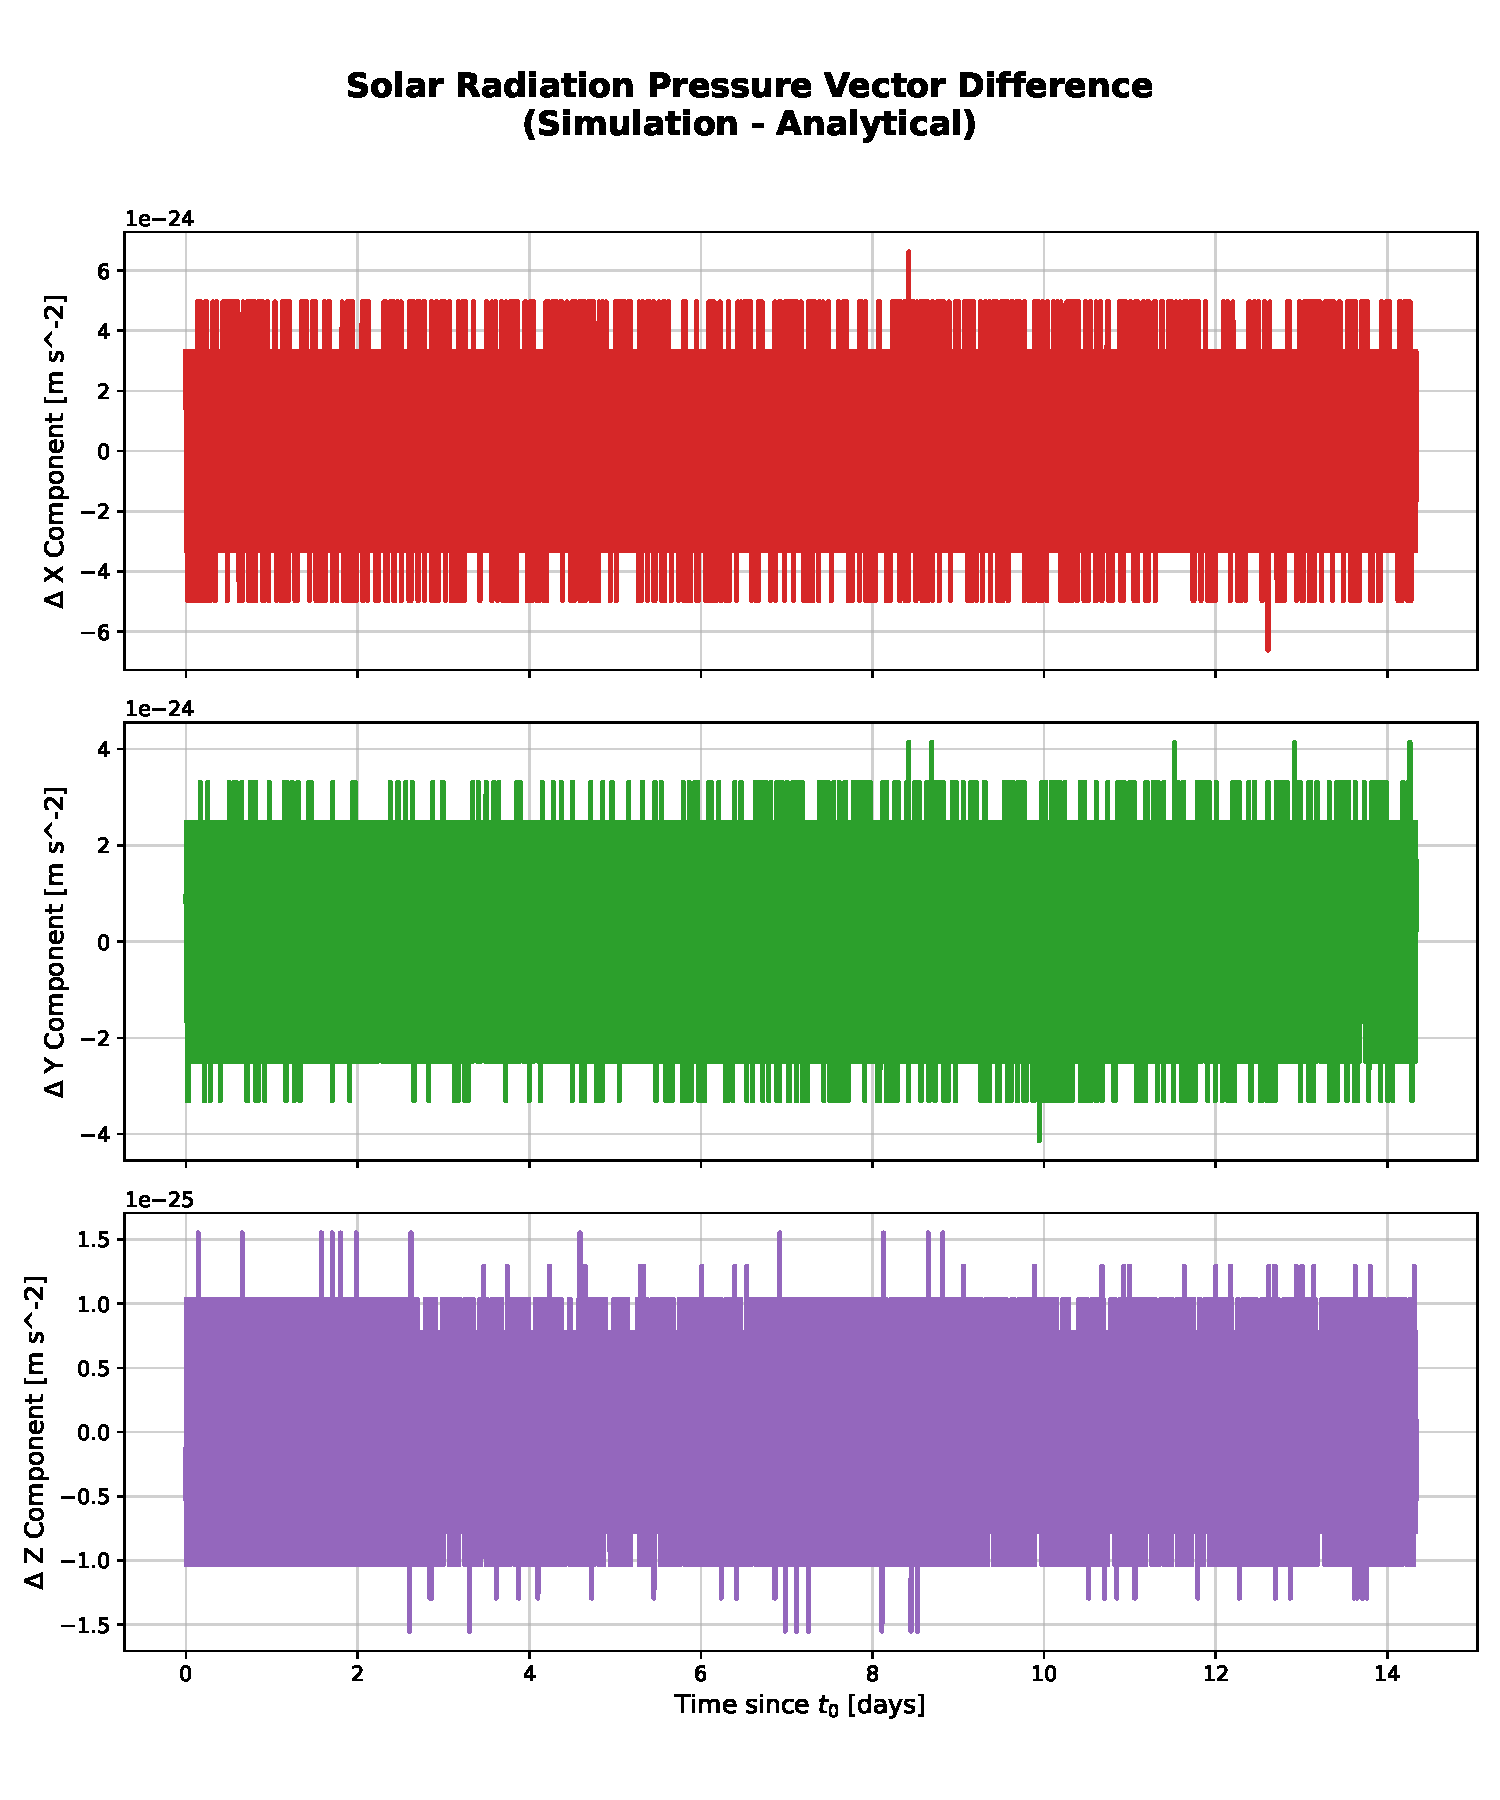
\includegraphics[width=0.85\textwidth]{../../figures/validation_srp_vector_diff_q3.pdf}
    \caption{Difference in Ganymede-centered Solar Radiation Pressure acceleration vector acting on JUICE, between manually calculated and extracted from propagation.}
    \label{fig:validation_srp_vector_diff_q3}
\end{figure}

\autoref{fig:aero_mag_diff_q3}, \ref{fig:aero_vector_diff_q3}, \ref{fig:validation_srp_mag_diff_q3}, and \ref{fig:validation_srp_vector_diff_q3} show that the manually calculated accelerations match the extracted propagation values within numerical precision. 

\subsection*{b}

\begin{figure}[H]
    \centering
    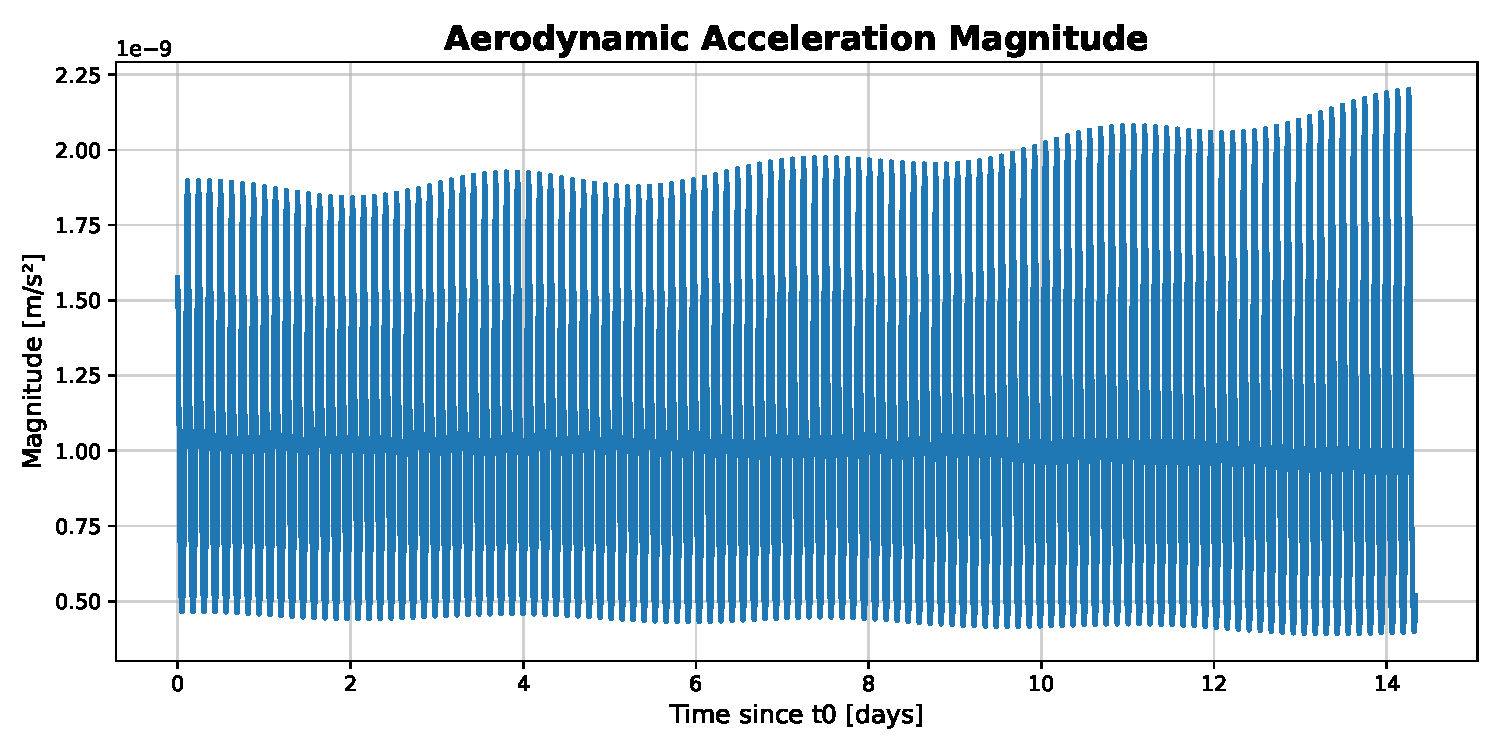
\includegraphics[width=0.85\textwidth]{../../figures/rsw_aero_acceleration_magnitude_q3.pdf}
    \caption{Ganymede-centered aerodynamic acceleration magnitude acting on JUICE, in RSW frame.}
    \label{fig:rsw_aero_acceleration_magnitude_q3}
\end{figure}

\begin{figure}[H]
    \centering
    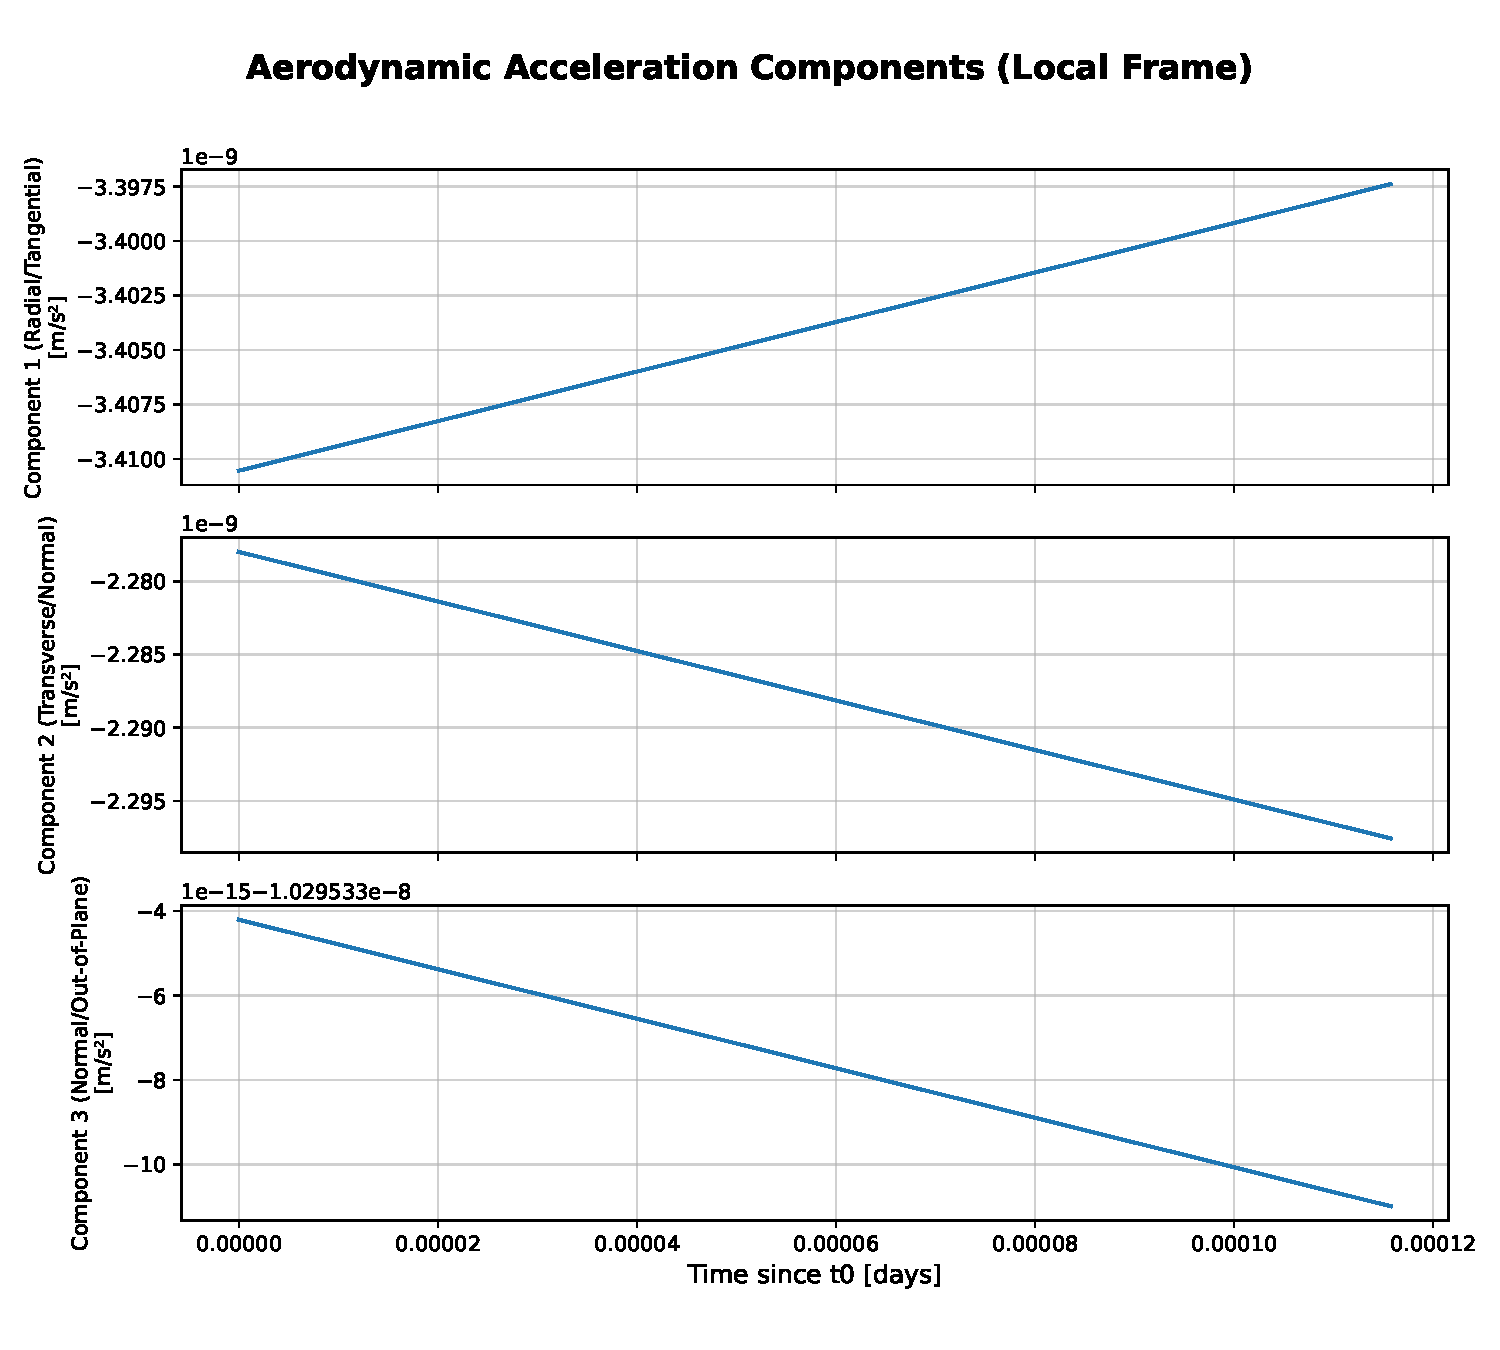
\includegraphics[width=0.85\textwidth]{../../figures/rsw_aero_acceleration_vector_local_q3.pdf}
    \caption{Ganymede-centered aerodynamic acceleration vector acting on JUICE, RSW frame.}
    \label{fig:rsw_aero_acceleration_vector_local_q3}
\end{figure}

\begin{figure}[H]
    \centering
    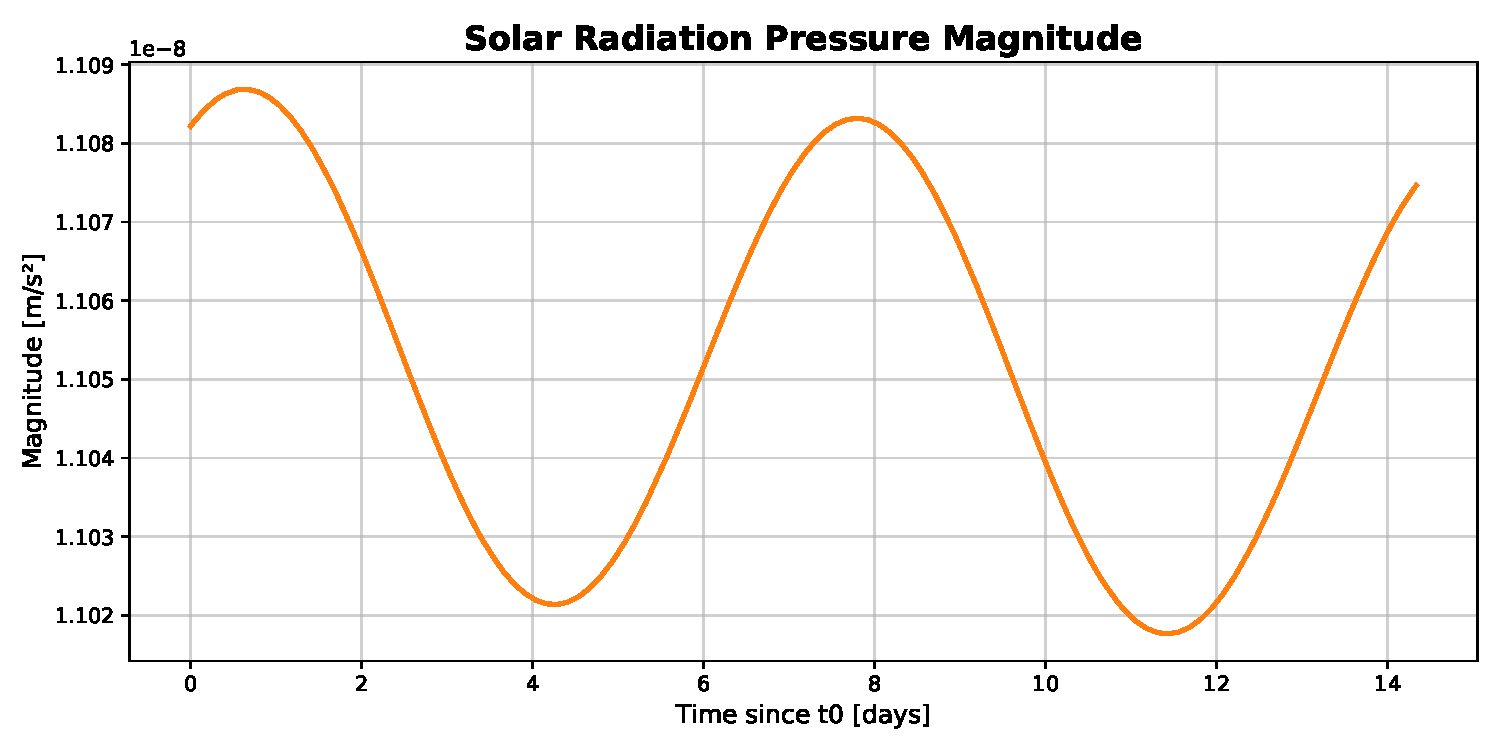
\includegraphics[width=0.85\textwidth]{../../figures/rsw_srp_acceleration_magnitude_q3.pdf}
    \caption{Ganymede-centered Solar Radiation Pressure acceleration magnitude acting on JUICE, in RSW frame}
    \label{fig:rsw_srp_acceleration_magnitude_q3}
\end{figure}

\begin{figure}[H]
    \centering
    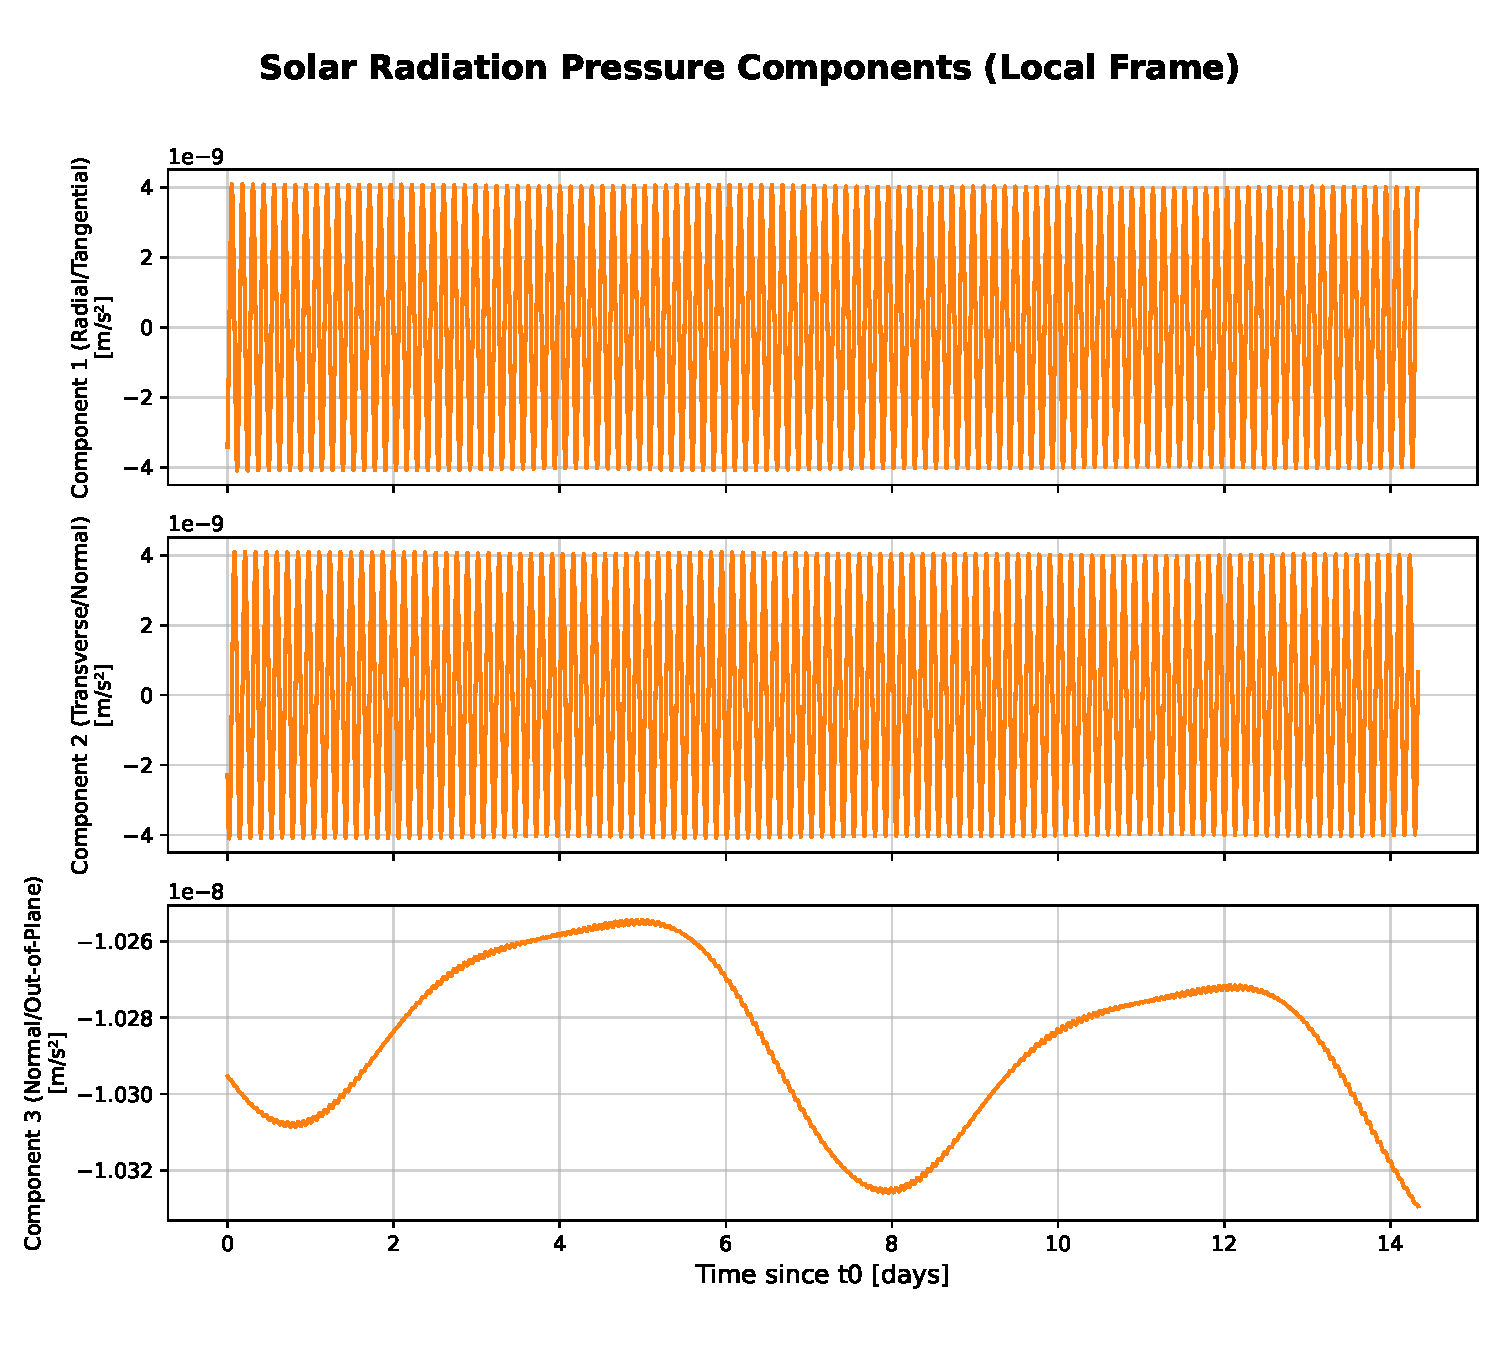
\includegraphics[width=0.85\textwidth]{../../figures/rsw_srp_acceleration_vector_local_q3.pdf}
    \caption{Ganymede-centered Solar Radiation Pressure acceleration vector acting on JUICE, RSW frame.}
    \label{fig:rsw_srp_acceleration_vector_local_q3}
\end{figure}

\subsection*{c.i}

\begin{figure}[H]
    \centering
    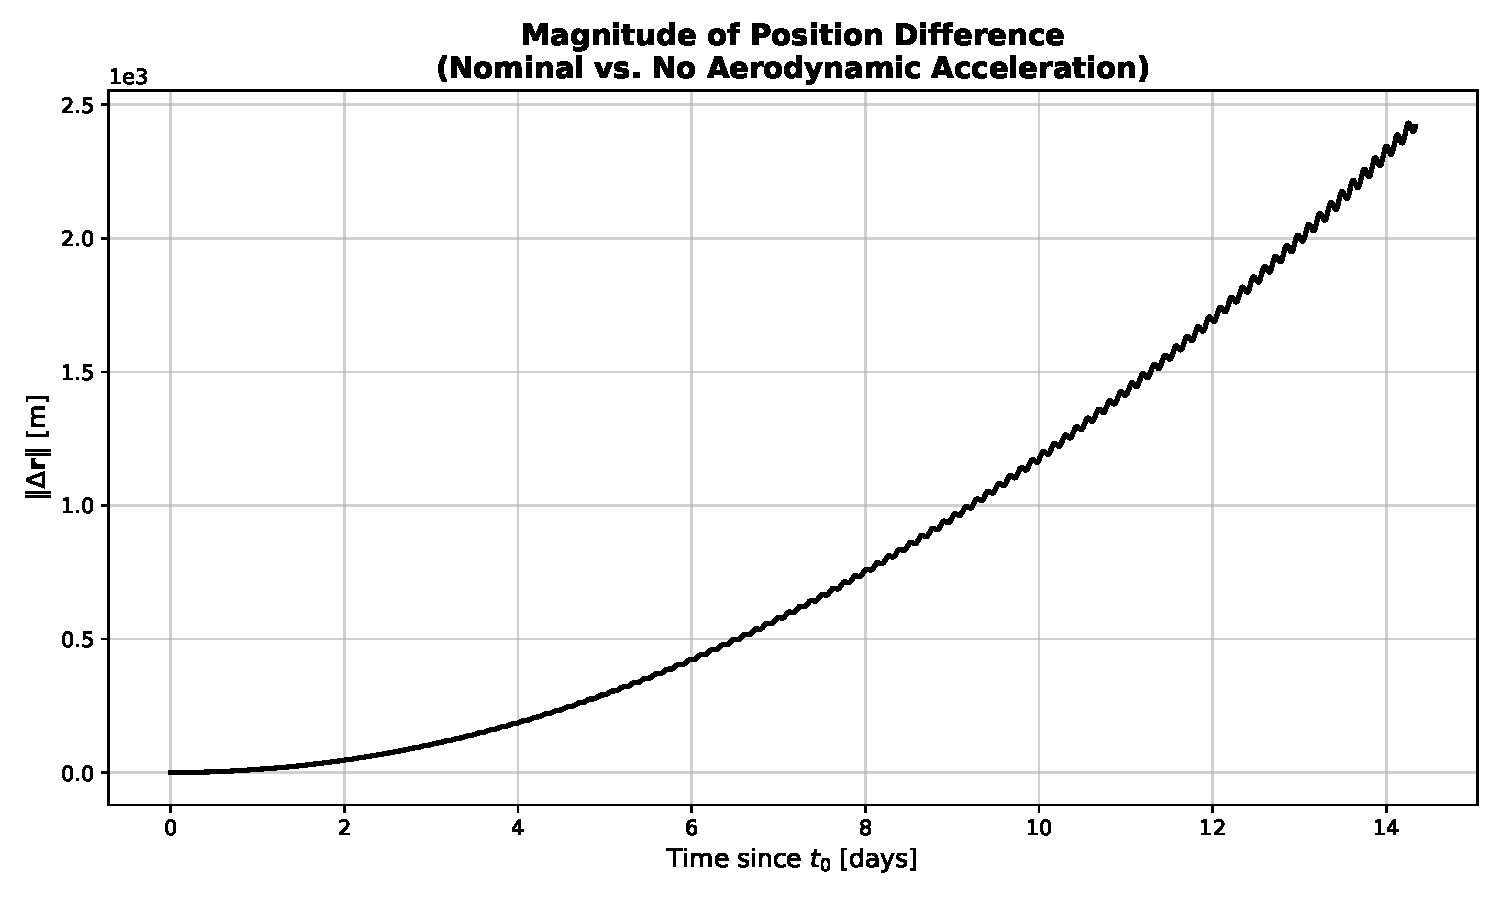
\includegraphics[width=0.85\textwidth]{../../figures/position_difference_magnitude_aero_effect_q3.pdf}
    \caption{Norm of the difference between the position of JUICE obtained from the nominal propagation and the propagation without aerodynamic acceleration.}
    \label{fig:position_difference_magnitude_aero_effect_q3}
\end{figure}

\begin{figure}[H]
    \centering
    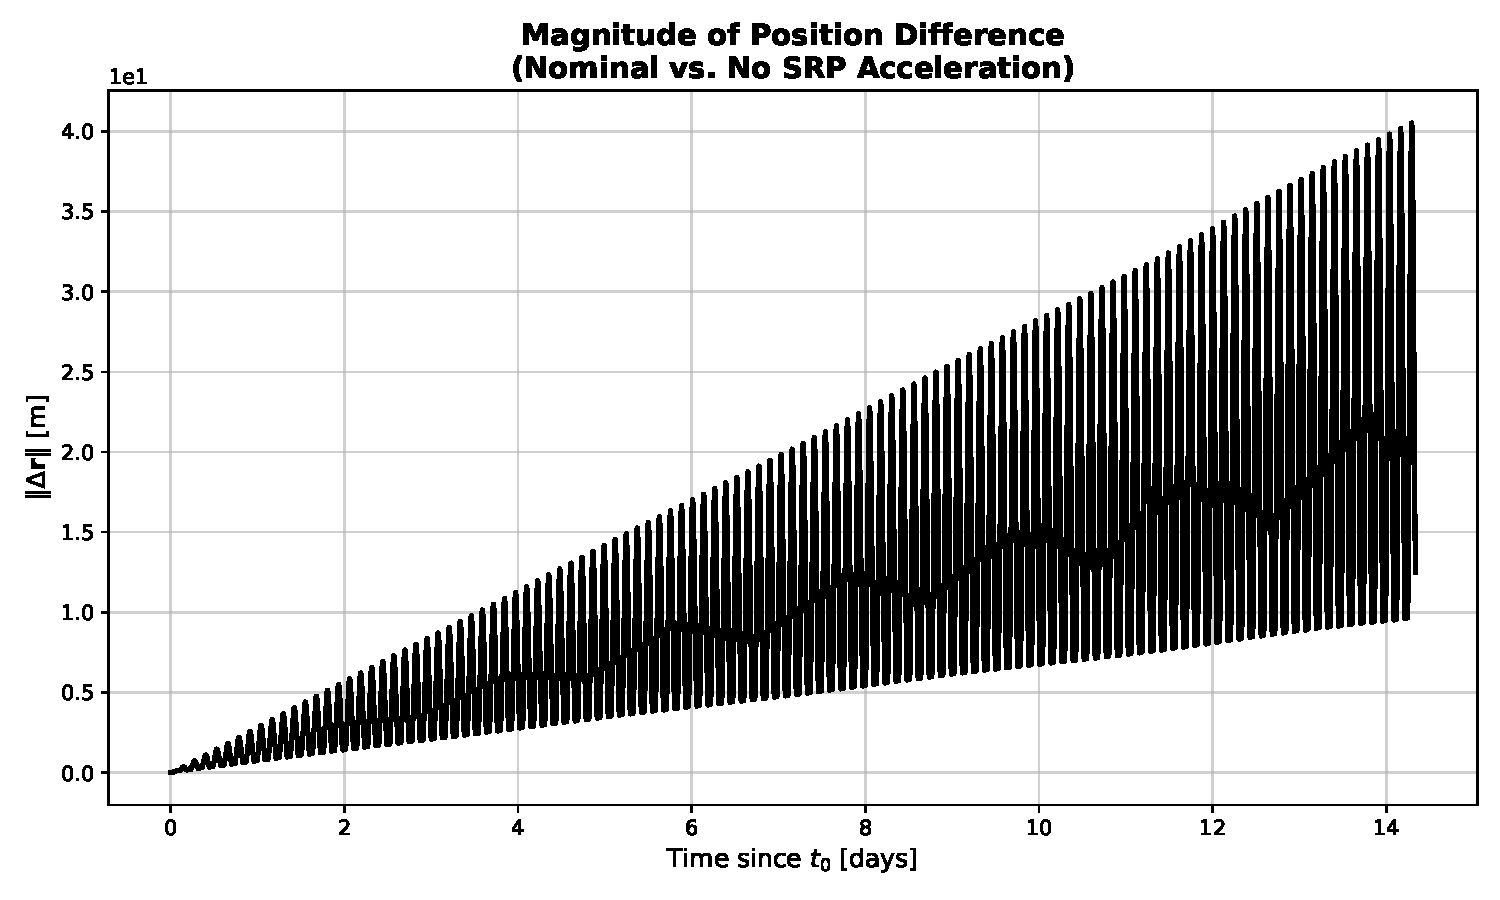
\includegraphics[width=0.85\textwidth]{../../figures/position_difference_magnitude_srp_effect_q3.pdf}
    \caption{Norm of the difference between the position of JUICE obtained from the nominal propagation and the propagation without SRP acceleration.}
    \label{fig:position_difference_magnitude_srp_effect_q3}
\end{figure}

\subsection*{c.ii}
% \textit{\textbf{Explanation for stronger relative influence of aerodynamic acceleration on $||\Delta \mathbf{r}_{G,s}(t)||$}}.
As per \autoref{fig:position_difference_magnitude_aero_effect_q3} and \ref{fig:position_difference_magnitude_srp_effect_q3}, the aerodynamic acceleration has a stronger influence on the position difference than the SRP acceleration. 
From \autoref{fig:rsw_aero_acceleration_vector_local_q3}, in opposition to \autoref{fig:rsw_srp_acceleration_vector_local_q3}, it can be perceived that the aerodynamic acceleration has a bigger continuous effect in the along track direction, hence affecting the SMA during all the propagation.
Even though the SRP acceleration magnitude its greater, its long-term effects are less important because the in-plane components are periodic and quasi-symmetric, hence compensating the effect in long-term propagation (as this case).

\clearpage



\section*{Question 4}

\subsection*{a}
Assuming point-mass acceleration from Jupiter:
\begin{align*}
    {\left(\mathbf{a}_{s}\right)_{J}} 
    & = - \frac{\mu_J}{\|\mathbf{r}_{Js}\|^3} \mathbf{r}_{Js} - \frac{\mu_G}{\|\mathbf{r}_{Gs}\|^3} \mathbf{r}_{Gs} + \frac{\mu_G}{\|\mathbf{r}_{GJ}\|^3} \mathbf{r}_{GJ} \\
    & = - \frac{\mu_J}{\|\mathbf{r}_{Js}\|^3} \mathbf{r}_{Js} - \frac{\mu_G}{\|\mathbf{r}_{GJ} + \mathbf{r}_{Js}\|^3} (\mathbf{r}_{GJ} + \mathbf{r}_{Js}) + \frac{\mu_G}{\|\mathbf{r}_{GJ}\|^3} \mathbf{r}_{GJ} 
\end{align*}
where $\left(\mathbf{a}_{s}\right)_{J}$ is the Jupiter-centered acceleration of JUICE, $\mu_J$ is the gravitational parameter of Jupiter, $\mathbf{r}_{Js}$ is the position vector from Jupiter to JUICE, $\mu_G$ is the gravitational parameter of Ganymede, $\mathbf{r}_{Gs}$ is the position vector from Ganymede to JUICE, and $\mathbf{r}_{GJ}$ is the position vector from Ganymede to Jupiter.

\begin{figure}[H]
    \centering
    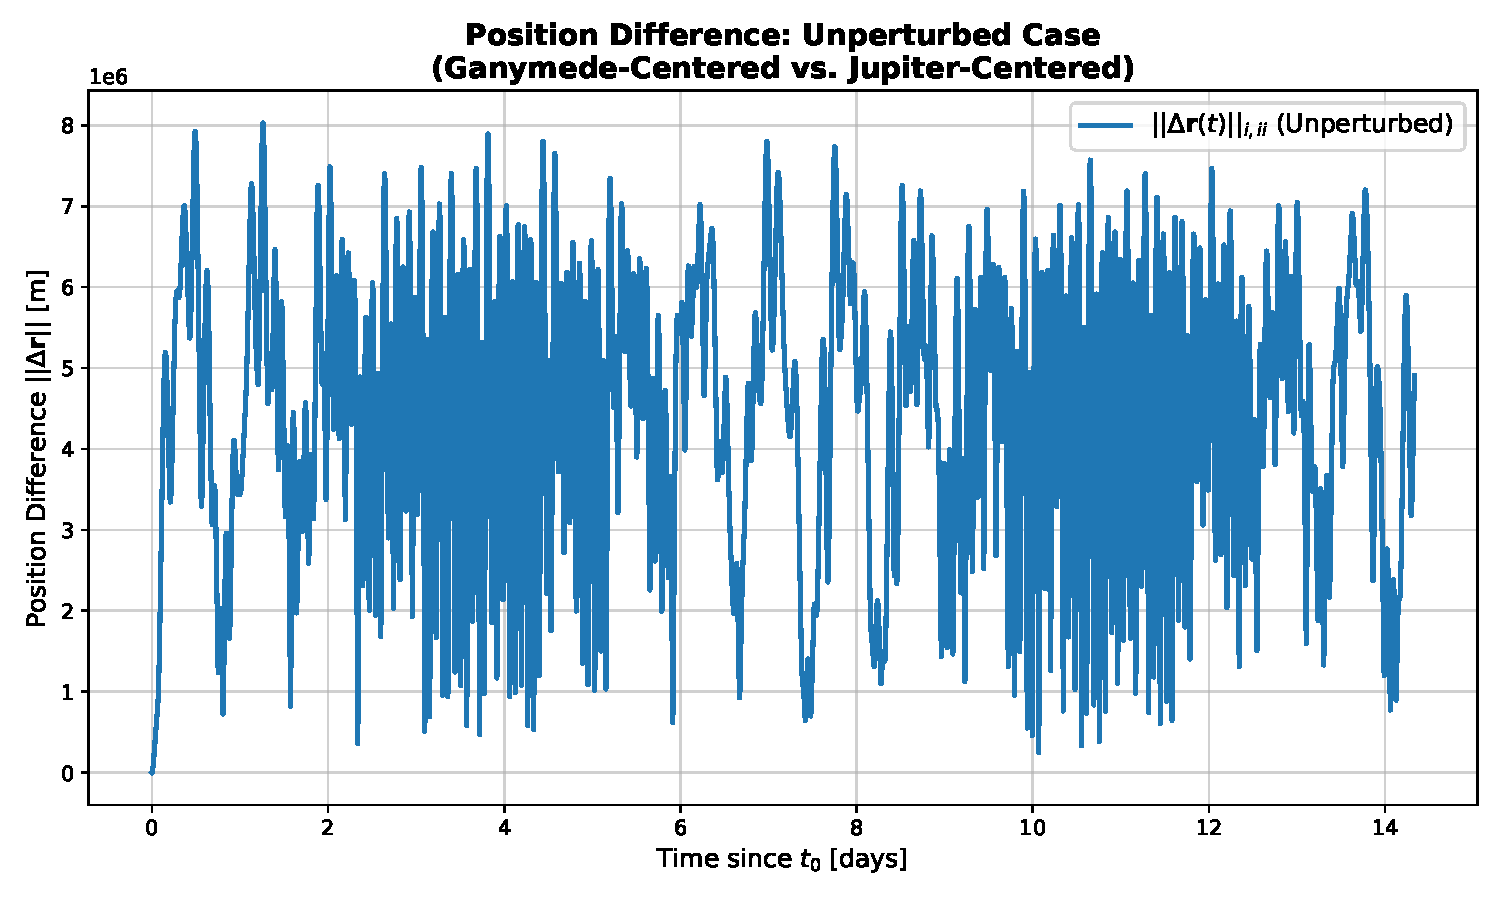
\includegraphics[width=0.85\textwidth]{../../figures/propagation_origin_unperturbed_q4.pdf}
    \caption{Magnitude of the difference in position for the Ganymede-centered and Jupiter-centered unperturbed propagations.}
    \label{fig:propagation_origin_unperturbed_q4}
\end{figure}

\subsection*{b}
\begin{align*}
    & \left(\mathbf{a}_{G,s}\right)_{J} = \nabla U_G(\mathbf{r}_{Gs}) - \nabla U_G(\mathbf{r}_{GJ}) = \nabla U_G(\mathbf{r}_{GJ} + \mathbf{r}_{Js}) - \nabla U_G(\mathbf{r}_{GJ}) \\
    & \left(\mathbf{a}_{J,s}\right)_{J} = \nabla U_J(\mathbf{r}_{Js}) \\% = \nabla U_J(\mathbf{r}_{JG} + \mathbf{r}_{Gs}) \\
    & \left(\mathbf{a}_{I,s}\right)_{J} = - \mu_I \frac{\mathbf{r}_{Is}}{\|\mathbf{r}_{Is}\|^3} + \mu_I \frac{\mathbf{r}_{IJ}}{\|\mathbf{r}_{IJ}\|^3} = -\mu_I \left( \frac{\mathbf{r}_{IG} + \mathbf{r}_{Gs}}{\|\mathbf{r}_{IG} + \mathbf{r}_{Gs}\|^3} - \frac{\mathbf{r}_{IJ}}{\|\mathbf{r}_{IJ}\|^3} \right)
\end{align*}
where $\left(\mathbf{a}_{G,s}\right)_{J}$ is the Jupiter-centered acceleration of JUICE due to Ganymede, $U_G$ is the gravitational potential of Ganymede, $\mathbf{r}_{Gs}$ is the position vector from Ganymede to JUICE, $\mathbf{r}_{GJ}$ is the position vector from Ganymede to Jupiter, $\mathbf{r}_{Js}$ is the position vector from Jupiter to JUICE, $\left(\mathbf{a}_{J,s}\right)_{J}$ is the Jupiter-centered acceleration of JUICE due to Jupiter, $U_J$ is the gravitational potential of Jupiter, $\left(\mathbf{a}_{I,s}\right)_{J}$ is the Jupiter-centered acceleration of JUICE due to Io, $\mu_I$ is the gravitational parameter of Io, $\mathbf{r}_{Is}$ is the position vector from Io to JUICE, $\mathbf{r}_{IJ}$ is the position vector from Io to Jupiter, and $\mathbf{r}_{IG}$ is the position vector from Io to Ganymede.

\begin{figure}[H]
    \centering
    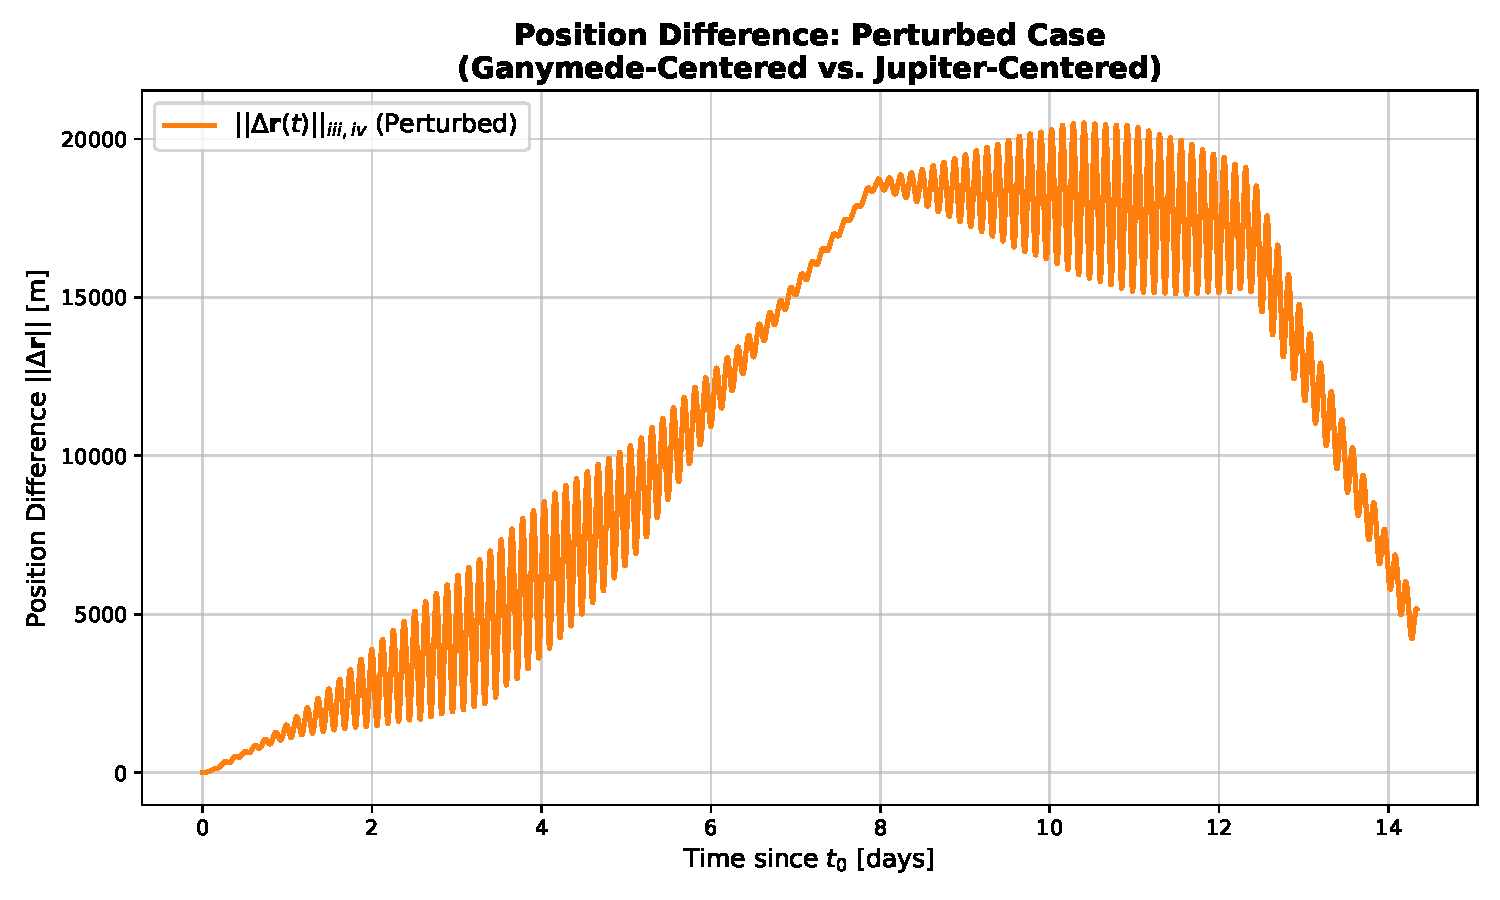
\includegraphics[width=0.85\textwidth]{../../figures/propagation_origin_perturbed_q4.pdf}
    \caption{Magnitude of the difference in position for the Ganymede-centered and Jupiter-centered perturbed propagations.}
    \label{fig:propagation_origin_perturbed_q4}
\end{figure}

\subsection*{c}

% \textit{\textbf{Provide physical and mathematical explanation for the observed behavior}. Add figures, tables, equations, etc. to support your reasoning. Captions of these (including definition of terms in equations) do not count towards the line limit (within reason).}

The SPICE ephemeris for Ganymede inherently includes all significant gravitational perturbations acting on it: $J_2$ and third-body effects. This represents the most accurate model available.

For cases $i$ and $ii$, the acceleration model in \textbf{4a} includes only point-mass gravity from Jupiter and Ganymede. Specifically, this model is missing: Jupiter's $J_2$ gravitational harmonics; third-body perturbations from Io, Europa, and the Sun; Ganymede's gravitational harmonics (point-mass only).

Since Ganymede's  SPICE ephemeris was generated using these missing perturbations, but our propagation neglects them, the two reference frames diverge significantly. This mathematical inconsistency directly manifests as the large $||\Delta \mathbf{r}(t)||_{i,ii}$ shown in \ref{fig:propagation_origin_unperturbed_q4}.

In contrast, for cases $iii$ and $iv$, the acceleration model in \textbf{4b} includes Jupiter's full $\nabla U_J$, Ganymede's potential $\nabla U_G$, and Io's third-body effects. While still missing the Sun and Europa, this model captures the dominant perturbations present in the SPICE ephemeris. Consequently, our propagated Ganymede trajectory more closely approximates the SPICE reality, resulting in the much smaller $||\Delta \mathbf{r}(t)||_{iii,iv}$ observed in \ref{fig:propagation_origin_perturbed_q4}.

The reduction from the unperturbed to the perturbed case confirms that including more realistic dynamics in the propagation reduces the inconsistency between numerical integration and SPICE ephemerides.


\subsection*{d}

\begin{figure}[H]
    \centering
    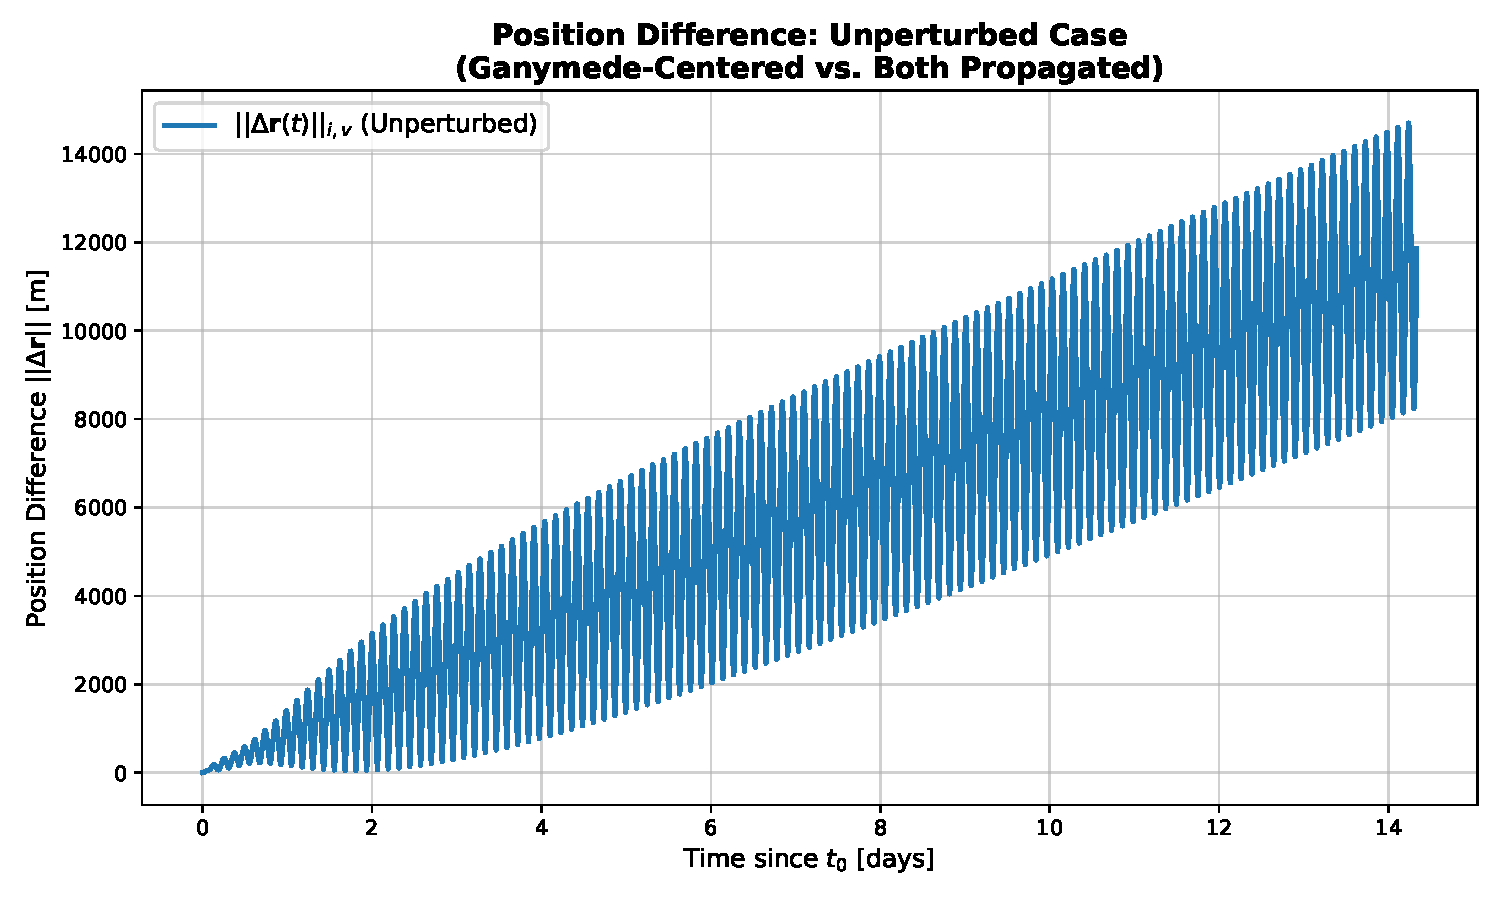
\includegraphics[width=0.85\textwidth]{../../figures/propagation_origin_unperturbed_d_q4.pdf}
    \caption{Magnitude of the difference in position for the Ganymede-centered and Jupiter-centered unperturbed propagations, also propagating Ganymede.}
\end{figure}

\begin{figure}[H]
    \centering
    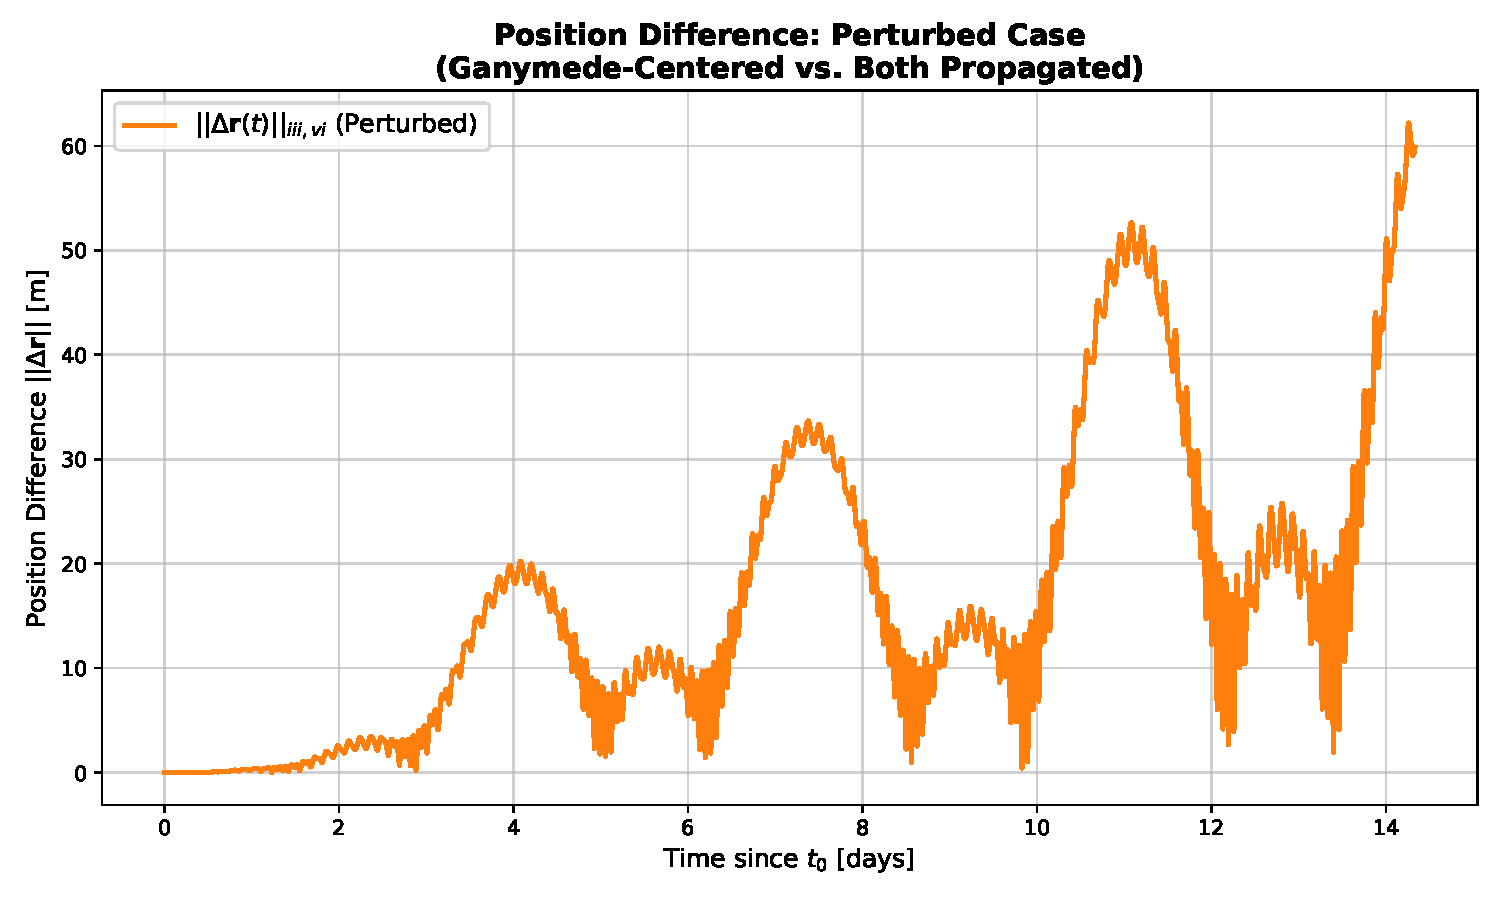
\includegraphics[width=0.85\textwidth]{../../figures/propagation_origin_perturbed_d_q4.pdf}
    \caption{Magnitude of the difference in position for the Ganymede-centered and Jupiter-centered perturbed propagations, also propagating Ganymede.}
\end{figure}

% \textit{\textbf{Explain why your results here (dis)prove the hypothesis you formulated in question c}. Add figures, tables, equations, etc. to support your reasoning. Captions of these (including definition of terms in equations) do not count towards the line limit (within reason).}

The results confirm the hypothesis formulated in \textbf{c} through the principle of dynamical consistency. 

By propagating Ganymede numerically using the exact same force model applied to JUICE, both bodies now exist within the same simplified mathematical universe. 

In contrast, when Ganymede's position is extracted from SPICE (\textbf{a} and \textbf{b}), it represents the "real" high-fidelity universe that includes all perturbations. The JUICE trajectory, however, is computed in a simplified universe. This mismatch between reference frames causes the massive artificial drift observed in \ref{fig:propagation_origin_unperturbed_q4} and \ref{fig:propagation_origin_perturbed_q4}.

When both bodies are propagated with consistent dynamics, this artificial drift vanishes. $||\Delta \mathbf{r}(t)||$ now reflects only numerical integration errors and frame transformation precision. This validates that the large errors in parts \textbf{a--c} arise from referencing an inconsistent dynamical framework, not from inherent inaccuracies in the propagation scheme itself.


\end{document}
